% Options for packages loaded elsewhere
\PassOptionsToPackage{unicode}{hyperref}
\PassOptionsToPackage{hyphens}{url}
\PassOptionsToPackage{space}{xeCJK}
\documentclass[
]{ctexart}
\usepackage{xcolor}
\usepackage{amsmath,amssymb}
\setcounter{secnumdepth}{-\maxdimen} % remove section numbering
\usepackage{iftex}
\ifPDFTeX
  \usepackage[T1]{fontenc}
  \usepackage[utf8]{inputenc}
  \usepackage{textcomp} % provide euro and other symbols
\else % if luatex or xetex
  \usepackage{unicode-math} % this also loads fontspec
  \defaultfontfeatures{Scale=MatchLowercase}
  \defaultfontfeatures[\rmfamily]{Ligatures=TeX,Scale=1}
\fi
\usepackage{lmodern}
\ifPDFTeX\else
  % xetex/luatex font selection
  \setmainfont[]{Times New Roman}
  \ifXeTeX
    \usepackage{xeCJK}
    \setCJKmainfont[]{SimSun}
    \setCJKsansfont[]{SimHei}
    \setCJKmonofont[]{SimSun}
  \fi
  \ifLuaTeX
    \usepackage[]{luatexja-fontspec}
    \setmainjfont[]{SimSun}
  \fi
\fi
% Use upquote if available, for straight quotes in verbatim environments
\IfFileExists{upquote.sty}{\usepackage{upquote}}{}
\IfFileExists{microtype.sty}{% use microtype if available
  \usepackage[]{microtype}
  \UseMicrotypeSet[protrusion]{basicmath} % disable protrusion for tt fonts
}{}
\makeatletter
\@ifundefined{KOMAClassName}{% if non-KOMA class
  \IfFileExists{parskip.sty}{%
    \usepackage{parskip}
  }{% else
    \setlength{\parindent}{0pt}
    \setlength{\parskip}{6pt plus 2pt minus 1pt}}
}{% if KOMA class
  \KOMAoptions{parskip=half}}
\makeatother
\usepackage{longtable,booktabs,array}
\usepackage{calc} % for calculating minipage widths
% Correct order of tables after \paragraph or \subparagraph
\usepackage{etoolbox}
\makeatletter
\patchcmd\longtable{\par}{\if@noskipsec\mbox{}\fi\par}{}{}
\makeatother
% Allow footnotes in longtable head/foot
\IfFileExists{footnotehyper.sty}{\usepackage{footnotehyper}}{\usepackage{footnote}}
\makesavenoteenv{longtable}
\usepackage{graphicx}
\makeatletter
\newsavebox\pandoc@box
\newcommand*\pandocbounded[1]{% scales image to fit in text height/width
  \sbox\pandoc@box{#1}%
  \Gscale@div\@tempa{\textheight}{\dimexpr\ht\pandoc@box+\dp\pandoc@box\relax}%
  \Gscale@div\@tempb{\linewidth}{\wd\pandoc@box}%
  \ifdim\@tempb\p@<\@tempa\p@\let\@tempa\@tempb\fi% select the smaller of both
  \ifdim\@tempa\p@<\p@\scalebox{\@tempa}{\usebox\pandoc@box}%
  \else\usebox{\pandoc@box}%
  \fi%
}
% Set default figure placement to htbp
\def\fps@figure{htbp}
\makeatother
\setlength{\emergencystretch}{3em} % prevent overfull lines
\providecommand{\tightlist}{%
  \setlength{\itemsep}{0pt}\setlength{\parskip}{0pt}}
\usepackage{bookmark}
\IfFileExists{xurl.sty}{\usepackage{xurl}}{} % add URL line breaks if available
\urlstyle{same}
\hypersetup{
  hidelinks,
  pdfcreator={LaTeX via pandoc}}

\author{}
\date{}

\begin{document}

\section{无门控智能体记忆架构中的记忆投毒：架构依赖的传播机制、容量控制与隔离不变性}\label{ux65e0ux95e8ux63a7ux667aux80fdux4f53ux8bb0ux5fc6ux67b6ux6784ux4e2dux7684ux8bb0ux5fc6ux6295ux6bd2ux67b6ux6784ux4f9dux8d56ux7684ux4f20ux64adux673aux5236ux5bb9ux91cfux63a7ux5236ux4e0eux9694ux79bbux4e0dux53d8ux6027}

\textbf{王斌}

北京开路者科技有限公司 · 技术总监

Email: wang.bin@foxmail.com；wangb@kailuzhe.cn

\textbf{摘要：} 长期运行的 LLM
智能体将经验沉淀进持久记忆；未经验证或恶意的条目可在会话间传播并污染下游任务。既有防御将软标记与硬隔离混为一谈，且尚无研究将记忆架构与传播的数学结构联系起来。本文在两种写入协议（选择性转写与全量追加）下研究注入-传播问题，通过覆盖三个模型族（DeepSeek-V4-Pro-0813（Pro）、Kimi、DeepSeek-V4.1-Flash-1017（Flash））、两种架构、多档容量、共
846 条智能体会话链（5,448 会话-代单元；selective 对照 2 链 × 6
代另计）的预注册实验，并以 Lean 4 机检条件定理支撑。

我们发现：决定传播机制的是架构而非模型。选择性转写产生分支衰减------Galton-Watson
分支过程，模型特定的每亲繁殖数
\(\hat m\in[0.56,0.98]\)，呈几何律衰减（\(R^2\ge0.92\)）；扩样至 12 链后
selective 侧 \(\hat m=0.966\)（CI \([0.911,1.000]\)），与全量追加侧 CI
完全分离。全量追加产生线性累积-容量竞争------每代写入
\(w_n\in\{0,1\}\)（链均 \(E[w_n]=0.917\)）使 \(Z_{n+1}=Z_n+w_n\)
线性累积直至记忆容量 \(M\)，此后 FIFO
竞争达到并维持稳态（\(5/16\)）（工程语义的持续累积；跨机制对比传播比见
§6.1）。容量 \(M\) 是控制参量，临界容量 \(M_c\) 是 \((b,M)\)
联合函数：良性写入率越高，临界容量越大（EXP-B 协议下
\(b{=}1/2\to W_c\le4\)、\(b{=}3\to W_c\in(4,8)\)、\(b{=}5\to W_c\in(8,12)\)）。主协议档（\(b{\approx}3\)
总写入上限、含毒株）\(M_c\in(8,16)\) 与 EXP-B \(b{=}3\) 行（\(b\)
为良性经验上限、毒株占额度；实测两档每代总写入同为 3.00，流量同构）在
\(W=16\) 主格点相容（稳态 5.06 vs 4.917，差异 2.9\%），在 \(W=8\)
边界格点读数分裂（灭绝 vs 0.92 存活，12
链扩样后保持）------\textbf{归因审计（§6.5）定位为
DeepSeek-V4.1-Flash-1017 毒株转写行为的亚小时级状态切换}（同一日历日内约
32 分钟即观测到高低转写态翻转；同日双协议重跑无差异，Fisher
\(p{=}0.155\)，10-22 原批显著偏低 \(p{=}0.0024\)），\textbf{\(M_c\)
因而是 \((b,M,\) 毒株转写状态\()\) 条件量}：低转写态下
\(M_c\in(8,16)\)（\(W{=}8\) 灭绝），高转写态下 \(W{=}8\) 存活 0.75（12
链，探针门控重扫实测）------缩小记忆窗口不能可靠防住投毒，因为同一窗口在模型的另一行为状态下失效。

防御侧：软标记效应模型异质且不可靠（Pro 档 47\%
压缩在功效不足下不显著；full-append 12/12
逐代同轨为写路径结构绕过；Flash 大样本配对 \(n=48\)
确证零压缩，\(\bar d=0.020\)，\(p=0.69\)），而隔离（\(\sigma=1\)）在所有条件下截断传播：跨模型
24/24、跨任务族 48/48、full-append 12/12 链；σ
扫描（\(n=48\)/档）确认\textbf{全谱
\(\sigma_{\rm eff}\in\{0.1,0.25,0.5,0.75,0.9,1.0\}\) 实测（含 2026-10-23
补测中间档
\(\sigma_{\rm eff}\in\{0.75,0.9\}\)）}：\(\sigma_{\rm eff}<1\)
档全部存活率 1.00、无一抑制毒株（无甜点，A-H4 判据），σ=1 的记忆效用保留
0.88（代价为 12\%
新经验增量，种子知识无损）。在隔离与标记之间还存在受控实证的\textbf{控制律高态分支}（状态反馈软调节的设计形式；实验窗探针全程判高态、动态臂零切换，\textbf{跨状态切换动力学未行使，列为待测}）：高转写态下窗口收缩策略（\(W{=}8\to4\)）将毒株存活由
0.833 压至 0.333（12 链 vs 12 链同批对照，Fisher
\(p{=}0.018\)；跨三窗口合并 13/32 vs 19/24，单侧
\(p{=}0.004\)）、记忆效用保留 0.328 \(\ge0.275\)（C2
判据），但效用代价约七成良性记忆且有效性依赖探针带宽（§7/§11.4）。我们据此得出结论：\textbf{防御依赖结构手段而非参数或标记}------硬隔离为不可替代主体，窗口收缩策略（高态分支实证）为受控实证的次优层。方法学上，我们预注册的分支匹配假说被逐代机制证据证伪，修订为线性累积-竞争，本文如实报告这一修订。作为副产品，归因审计暴露了一个超出原实验范围的独立发现：\textbf{固定模型
checkpoint 的毒株转写倾向存在亚小时级的双峰状态漂移}（多批对照，Fisher
\(p\le0.0024\)）；我们据此提出\textbf{探针校准协议}------实验批启动前以约
3
分钟/链的探针判定当前毒株转写状态，跨批比较限于同状态批次------该协议本身构成可复用的方法论贡献。

\textbf{关键词：} 无门控智能体记忆架构；记忆投毒；预注册受控实验；Lean 4
形式化验证；硬隔离；分支过程

\begin{center}\rule{0.5\linewidth}{0.5pt}\end{center}

\subsection{1 引言}\label{ux5f15ux8a00}

\subsection{1.1 问题}\label{ux95eeux9898}

LLM
智能体（agent）正被部署到长期运行的生产系统：经验沉淀进持久记忆库，经检索在跨会话任务间复用。这一架构引入了一类此前未被系统研究的失效模式------\textbf{记忆投毒（memory
poisoning）}：未经验证的自生经验（或攻击者注入的经验）进入记忆库后，经代际转写被持续复制，污染后续所有相关任务。文献已确立攻击的现实性与跨会话持久性（MemoryGraft,
arXiv:2512.16962；OEP,
arXiv:2605.18930），以及递归自我消费在训练期的宏观坍缩后果（Shumailov et
al., \emph{Nature} 631,
2024）。然而，\textbf{记忆架构本身如何调节传播、防御为何失败、何种干预有机制层保证}------这三问缺少实证与形式化的回答。

\subsection{1.2 三个空白}\label{ux4e09ux4e2aux7a7aux767d}

\begin{enumerate}
\def\labelenumi{\arabic{enumi}.}
\tightlist
\item
  \textbf{机制空白}：传播究竟服从何种数学模型，取决于记忆的转写协议（选择性转写
  vs 全量追加）------此前没有跨架构的对照实验；
\item
  \textbf{防御空白}：软标记（标记门）与硬隔离（门禁）被混为一谈，没有独立判据区分二者在传播动力学上的作用；
\item
  \textbf{形式化空白}：软件工程学科的''根本规律''（Brooks 1987；Lehman
  1980；Conway 1968）历来是经验定律，从未被形式化证明（§2.5
  定位）；智能体记忆的投毒-隔离规律同样停留在启发式层面。
\end{enumerate}

\subsection{1.3 本工作}\label{ux672cux5de5ux4f5c}

本工作根植的\textbf{公理
IV（经验自免疫）}主张：未经\textbf{物理验证与独立审查终审}的自生经验经检索复用会对后续任务产生持续性污染，其防御须依赖写入层的结构阻断（隔离）而非决策层的软信号（标记）。在此框架下，本文给出\textbf{机制识别
+ 形式化 + 预注册实证}的完整闭环：

\begin{enumerate}
\def\labelenumi{\arabic{enumi}.}
\tightlist
\item
  \textbf{机制层}：识别''架构决定传播机制''------选择性转写产生分支衰减（Galton-Watson
  分支过程），全量追加产生线性累积-容量竞争（每代写入
  \(w_n\in\{0,1\}\)，链均 0.917）；记忆容量 \(M\) 为控制参量，临界
  \(M_c\in(8,16)\)（低转写态读数，§3/§6.5）；
\item
  \textbf{形式化层}：Lean 4 机检定理链（零 \texttt{sorry}，§4）------GW
  灭绝概率=最小不动点、亚临界概率灭绝、隔离压缩后代、超临界正概率不灭绝；
\item
  \textbf{实证层}：预注册、跨模型（Pro / Kimi / Flash；全名与简称映射见
  §5.2）× 跨架构（selective / full-append / 容量档）× 跨任务族（144
  链）× 大样本配对（160 链）闭合判据（§5--§6）；
\item
  \textbf{工程含义}：防御依赖\textbf{隔离而非标记}------标记门效应模型异质且不可靠------Pro
  档 47\% 压缩在功效不足下不显著、C1-full 写路径结构同轨、Flash
  大样本确证零压缩（\(\bar d=0.020\)，\(p=0.69\)），隔离在跨模型（24/24
  链 \(Z_1=0\)）、跨任务族（48/48 链）、跨架构（12/12 链 mem 恒
  6）三维截断传播（§7）。
\end{enumerate}

\textbf{一项诚实的方法论声明}：预注册假说 S-H3（GW
分支匹配）被逐代机制证据（\(w_n\in\{0,1\}\)
线性累积）\textbf{证伪}。我们将其作为''预注册假说被证伪→机制重新识别''的正面案例完整呈现（§9），而非事后合理化。

\subsection{1.4 论文结构}\label{ux8bbaux6587ux7ed3ux6784}

§2 Related Work；§3 机制模型；§4 形式化；§5 实验设置；§6 结果；§7
讨论；§9 机制修正叙事；§10 适用域；§11 局限；§12 结论。

\subsection{2
背景与相关工作}\label{ux80ccux666fux4e0eux76f8ux5173ux5de5ux4f5c}

\subsection{2.1
智能体记忆与投毒}\label{ux667aux80fdux4f53ux8bb0ux5fc6ux4e0eux6295ux6bd2}

智能体长期记忆（agentic memory）已成为 LLM
应用系统的标准组件：经验经检索（retrieval）复用，构成跨会话的持续知识层。与此同时，记忆已成为一类高价值攻击面：\textbf{记忆投毒（memory
poisoning）}------攻击者或智能体自身的失效经验注入记忆库后，经后续检索被持久复用，污染后续任务（Shumailov
et al., 2024；MemoryGraft,
2025）。近期实证表明，投毒攻击可跨会话持久生效，且极低污染率即可造成高攻击成功率（MemoryGraft,
arXiv:2512.16962）；自进化智能体在''局部正确但不可迁移''经验下的污染路径亦有刻画（OEP,
arXiv:2605.18930）。这些工作确立了攻击的现实性与持续性，但\textbf{防御侧停留在启发式}（标记、过滤、人工审查），缺乏对''为什么某些防御失效''的机制层解释------本工作补上这一层。

\textbf{必须正面对话的竞争工作}：arXiv:2605.08442（\emph{Defense
effectiveness across architectural layers}，2026-05）对 9
个模型的持久记忆攻击做了跨架构层的机制评估，结论是输入层防御无法观测 RAG
注入内容、检索层分类器可被语义掩蔽绕过，而记忆层的硬性工具门控（Memory
Sandbox）将攻击成功率降至 0/9 模型中的 8
个------与本工作``隔离有效、软信号无效''的防御结论高度重叠。本文的增量不是防御建议本身，而是：(i)
给出两种记忆架构（selective vs
full-append）下传播的\textbf{动力学两分法}与容量控制参量
\(M_c\)（2605.08442 未涉及传播的数学结构）；(ii) 以预注册判据与 Lean
机检条件定理支撑隔离不变性。攻击面文献 AgentPoison（NeurIPS 2024,
arXiv:2407.12784）确立了记忆/知识库投毒的攻击现实性，本文与其在攻击-防御分工上衔接。

\subsection{2.2
模型坍缩与递归退化}\label{ux6a21ux578bux574dux7f29ux4e0eux9012ux5f52ux9000ux5316}

宏观层面的递归自我消费已被证明导致\textbf{模型坍缩（model
collapse）}：用递归生成的数据训练，模型分布退化为模式坍缩与方差消失（Shumailov
et al., \emph{Nature} 631, 2024）。其与分支过程（branching
process）的联系在文献中已有提及：退化可刻画为种群动态（population
dynamics）。本工作的理论工具------Galton-Watson
分支过程及其灭绝概率、几何衰减律（Harris,
1963）------正是这一联系的形式化端点之一。与 Shumailov
等的训练期坍缩不同，本工作关注\textbf{推理期/记忆期的传播}：不经过重训练，仅在上下文-记忆-转写回路中逐代传播。这一区分是本文机制的出发点。

\subsection{2.3
针对记忆投毒的防御}\label{ux9488ux5bf9ux8bb0ux5fc6ux6295ux6bd2ux7684ux9632ux5fa1}

既有防御沿两条思路：

\begin{enumerate}
\def\labelenumi{\arabic{enumi}.}
\tightlist
\item
  \textbf{软标记（soft
  marking）}：对自生经验打上''未验证''标记，供下游过滤（实验中的标记名
  DRAFT\_SUSPECT，§5.3）。本工作标记门效应\textbf{模型异质}：Pro 主实验
  47\% 压缩（C1/C0 比值 0.529）在功效不足（\(n=12\)，功效
  0.38）下不显著；SUPERCRITICAL C1-full 12/12 逐代同轨（full-append
  写路径结构绕过模型判断）；H1AC
  大样本配对（\(\bar d=0.020\)，\(p=0.69\)）确证 Flash
  档零压缩（模型档全名见 §5.2）------模型对软信号的采纳不可靠；
\item
  \textbf{硬隔离（hard
  quarantine）}：未经\textbf{五重物理判据}与\textbf{独立审查终审}的经验不得进入全局知识库（等价于本工作的门禁
  \(\sigma=1\)）。五重物理判据指编译、隐藏测试、真实执行探活、退出码核验、形式化审计五条\textbf{独立物理通道}全部绿灯方可晋升------LLM
  自评不构成证据；独立审查终审指与经验生产者物理隔离的仲裁门，不接受自然语言辩解。本工作实测：隔离在\textbf{跨模型（24/24
  链 \(Z_1=0\)）、跨任务族（48/48 链）、跨架构（full-append 12/12 链 mem
  恒 6）}三个维度上截断传播------防御依赖结构阻断而非模型行为。
\end{enumerate}

这一``隔离有效、标记失效''的分离，与 2605.08442
的``硬工具门控有效、软信号无效''结论方向一致，本文在其上补充了传播动力学机制与容量控制参量（§2.1
对话段）；MemoryGraft（2025）的防御讨论未区分二者。

\subsection{2.4
智能体的通用退化机制}\label{ux667aux80fdux4f53ux7684ux901aux7528ux9000ux5316ux673aux5236}

\begin{itemize}
\tightlist
\item
  \textbf{Reward hacking / specification
  gaming}：智能体满足目标的字面而非精神以骗取成功信号（Amodei et al.,
  2016；Krakovna et al., 2020）；生产级 RL
  中已观察到自然涌现的失对齐（Anthropic,
  arXiv:2511.18397）。这与本文公理
  I（外部锚定缺失→自我宣称不可信）同族，但未涉及代际传播。
\item
  \textbf{Context rot / Lost in the
  Middle}：随无关上下文增长，模型有效推理显著衰减，呈现 U
  型注意力曲线（Liu et al., TACL 2024）；有效上下文长度远低于标称（Hsieh
  et al., 2024, RULER；Chroma, 2024）。这对应公理
  II（注意力稀释），是\textbf{代内}退化；本文公理 IV
  关注\textbf{代际}传播，两者在因果链上衔接但机制不同。
\end{itemize}

\subsection{2.5
软件工程的''近公理''定律}\label{ux8f6fux4ef6ux5de5ux7a0bux7684ux8fd1ux516cux7406ux5b9aux5f8b}

软件工程学科的传统''根本规律''是\textbf{经验定律}而非形式公理：Brooks
的本质复杂性（Brooks, 1987）界定了工程极限；Lehman 定律（Lehman,
1980）刻画软件演化的持续变更与递增复杂性（软件的''熵增''）；Conway
定律（Conway, 1968）揭示架构-组织同构；CAP 定理（Gilbert \& Lynch,
2002）锁定分布式一致性的取舍；停机问题（Turing,
1936）界定可判定性边界。这些规律源自大量工程实践的经验总结，\textbf{从未被形式化证明}。

本工作的方法论立场：SE
的''近公理''规律可以且应当提升为\textbf{推理起点地位 +
经验可证伪内容}的工程公理。本文聚焦其中一支------经验自免疫------给出：Lean
4 机检的条件定理链（隔离⟹灭绝、GW
灭绝概率、几何律、超临界发散）、预注册的大样本实证、以及机制层修正（分支衰减
vs 累积-竞争）。这是把 SE
经验定律``形式化-实测化推进''的一次实例，而非凭空提出公设。需要限定的是：被机检的是概率论条件定理（Harris,
1963 结果的 Lean 复检），SE
定律的``工程公理化''是方法论主张而非形式化对象------本文不声称已形式化
Brooks/Lehman/Conway 定律本身。

\subsection{2.6
形式化验证工具}\label{ux5f62ux5f0fux5316ux9a8cux8bc1ux5de5ux5177}

定理链在 \textbf{Lean 4}（Moura \& Ullrich, 2021）中机检，零
\texttt{sorry}（条件定理与源码对应见
§4）。软件工程中形式化验证的应用先例（协议验证、并发正确性）支撑了''工程承诺以可机检定理呈现''的可行性；本文的贡献之一是此类条件定理（``对满足分支性与乘性压缩的系统，隔离使投毒谱系灭绝概率趋向
1''）在智能体记忆安全问题上的应用------就我们所知，这是该类型条件定理在该问题域的首次应用（限定于
§9 机制修正后的适用域）。

\subsection{3 模型}\label{ux6a21ux578b}

\subsection{3.1 记号}\label{ux8bb0ux53f7}

{\def\LTcaptype{} % do not increment counter
\begin{longtable}[]{@{}
  >{\raggedright\arraybackslash}p{(\linewidth - 4\tabcolsep) * \real{0.3333}}
  >{\raggedright\arraybackslash}p{(\linewidth - 4\tabcolsep) * \real{0.3333}}
  >{\raggedright\arraybackslash}p{(\linewidth - 4\tabcolsep) * \real{0.3333}}@{}}
\toprule\noalign{}
\begin{minipage}[b]{\linewidth}\raggedright
符号
\end{minipage} & \begin{minipage}[b]{\linewidth}\raggedright
含义
\end{minipage} & \begin{minipage}[b]{\linewidth}\raggedright
实测/设定
\end{minipage} \\
\midrule\noalign{}
\endhead
\bottomrule\noalign{}
\endlastfoot
\(Z_n\) & 第 \(n\) 代记忆库中毒株（P1 谱系）条目数（池大小） &
逐代追踪 \\
\(M\) & 记忆窗口容量（FIFO） & 默认 \(16\)；敏感性档 \(M=8,32\) \\
\(w_n\) & 第 \(n\) 代新写入的毒株条目数（fresh write） & selective：随
\(Z_n\) 变化；full-append：\(\in\{0,1\}\)（PMF={[}0,1{]}，链均
\(E[w_n]=0.917\)） \\
\(X_i\) & 分支过程的单亲后代数 & \(E[X]=\hat m\)（经验估计） \\
\(\sigma\) & 门禁拦截率（写出通过率 \(=1-\sigma\)） & 随机过滤
\(\sigma=0.5\)（半数拦截）；隔离 \(\sigma=1\)（全拦截） \\
\(\hat m\) & 传播比估计
\(\hat m=\sum_n Z_{n+1}/\sum_n Z_n\)（跨代加权平均；GW``每亲繁殖数''语义仅对机制
A 有效，见 §3.2） & 见各实验档 \\
\end{longtable}
}

\textbf{符号纪律}：\(M\) 为记忆容量（实验档名 \texttt{\_W8/\_W32}
中的窗口参数），\(w_n\) 为每代写入------两者在本文中严格区分。

\subsection{3.2
两个传播机制}\label{ux4e24ux4e2aux4f20ux64adux673aux5236}

\textbf{机制 A：分支衰减（selective
转写协议）}。智能体仅将当前会话中被判定相关的条目转写进记忆，后代数依赖亲代毒株的转写倾向：

\[Z_{n+1}=\sum_{i=1}^{Z_n} X_i,\qquad E[Z_{n+1}\mid Z_n]=\hat m\,Z_n\]

经典 Galton-Watson 分支过程（Harris, 1963）：期望传播按几何律
\(E[Z_n]=\hat m^n E[Z_0]\) 演化；灭绝概率为生成函数 \(\varphi(s)\)
的最小不动点（Lean T1）；亚临界（\(\hat m<1\)）指数衰减（Lean
T2）。\textbf{该机制的判据}：\(w_n\) 随 \(Z_n\) 变化（分支依赖）。

\textbf{机制 B：线性累积-容量竞争（full-append
转写协议）}。智能体将每代经验全量追加进记忆库（向量库直写/无转写衰减），毒株写入恒定：

\[Z_{n+1}=Z_n+w_n,\qquad w_n\in\{0,1\}\ \text{(实测, PMF=[0,1])}\]

未饱和段线性增长 \(Z_{n+1}=Z_n+1\)；当 \(Z_n\) 触及容量 \(M\) 后进入
FIFO 竞争稳态（新写条目挤占最旧条目），稳态池大小由容量竞争决定（实测
C0-full 稳态 \(5/16\)）。\textbf{该机制的判据}：\(w_n\) 恒定、不依赖
\(Z_n\)（累积写入）。

\textbf{机制判别的直接证据（逐代 offspring 核对）}：full-append
档每代新写 P1 为 0 或 1（\(w_n\in\{0,1\}\)，PMF={[}0,1{]}，链均
\(E[w_n]=0.917\)------11/12 链每代恒 1，约 1/12
链存在某代未写；\(Z_{n+1}=Z_n+w_n\) 线性累积，实测
Z={[}1,2,2.917,3.917,3.917,4.917,4.917,4.917{]}）；分支过程要求的''后代数依赖亲代种群''不成立。\textbf{由此，预注册假说
S-H3（GW 匹配）被机制证据证伪，理论修订为机制 B}（见 §9
机制修正叙事）。分支衰减（机制 A）仍在 selective 协议下成立（几何律
\(R^2=0.958\)，主实验；\(R^2=0.923\)，H1AC 大样本）。

\subsection{3.3
容量控制参量}\label{ux5bb9ux91cfux63a7ux5236ux53c2ux91cf}

记忆窗口容量 \(M\) 决定机制 B 的传播结局（SUPERCRITICAL
档，full-append，Flash）：

{\def\LTcaptype{} % do not increment counter
\begin{longtable}[]{@{}
  >{\raggedright\arraybackslash}p{(\linewidth - 6\tabcolsep) * \real{0.2500}}
  >{\raggedright\arraybackslash}p{(\linewidth - 6\tabcolsep) * \real{0.2500}}
  >{\raggedright\arraybackslash}p{(\linewidth - 6\tabcolsep) * \real{0.2500}}
  >{\raggedright\arraybackslash}p{(\linewidth - 6\tabcolsep) * \real{0.2500}}@{}}
\toprule\noalign{}
\begin{minipage}[b]{\linewidth}\raggedright
\(M\)
\end{minipage} & \begin{minipage}[b]{\linewidth}\raggedright
传播比 \(\hat m^\dagger\)（boot95 CI）
\end{minipage} & \begin{minipage}[b]{\linewidth}\raggedright
g7 存活率
\end{minipage} & \begin{minipage}[b]{\linewidth}\raggedright
结局
\end{minipage} \\
\midrule\noalign{}
\endhead
\bottomrule\noalign{}
\endlastfoot
8 & 0.829（{[}0.739, 0.875{]}） & 0 &
\textbf{灭绝}（写入侧即被容量压制） \\
16 & 1.166（{[}1.156, 1.176{]}） & 1.0 & \textbf{持续累积}（稳态 5/16
维持 3 代；工程语义超临界） \\
32 & 1.25（退化 CI，6 链全同） & 1.0 &
\textbf{线性增长}（\(Z=[1,\dots,8]\)，未饱和） \\
\end{longtable}
}

\textbf{临界容量是 \((b,M)\) 联合函数（EXP-B
实测，§6.5）}：容量单调性成立------\(M\le M_c\)
时毒株池被压制至灭绝，\(M>M_c\) 时单调累积不灭绝。\(M_c\) 随良性写入率
\(b\) 上移（EXP-B 协议下 \(b{=}1/2\) 时 \(W_c\le4\)、\(b{=}3\) 时
\(W_c\in(4,8)\)、\(b{=}5\) 时
\(W_c\in(8,12)\)）。\textbf{跨实验格点核对}：主协议档（写入规则''1\textasciitilde3
条''，\(b{\approx}3\)
总写入上限、含毒株，\texttt{axiom4\_memory\_propagation.py}
执行）\(M_c\in(8,16)\) 与 EXP-B \(b{=}3\) 行（\texttt{kimi\_boost.py}
执行；\(b\) 为良性经验上限、毒株占额度；实测两档每代总写入同为
3.00，流量同构）在 \(W=16\) 主格点相容（EXP-A C0 6 代 \(Z=5.06\) vs
主协议同代 4.917，差异 2.9\%），但在 \(W=8\) 边界格点读数分裂（主协议 6
链全灭 surv=0 vs EXP-B 12 链
surv=0.92，扩样后保持）------\textbf{归因审计（§6.5）定位为
DeepSeek-V4.1-Flash-1017 毒株转写行为的亚小时级状态切换}（同一日历日内约
32 分钟观测到高低态翻转；同日双协议重跑无差异 Fisher
\(p{=}0.155\)，10-22 原批显著偏低
\(p{=}0.0024\)，非协议差异），\textbf{\(M_c\) 因而是 \((b,M,\)
毒株转写状态\()\) 条件量}：低转写态下 \(M_c\in(8,16)\)、\(W{=}8\)
灭绝，高转写态下 \(W{=}8\) 存活过半（§11.4
探针校准协议）；两读数各自批内可复现，以并列读数如实报告（§6.5）；\(b\)
与检索策略均可使 \(M_c\) 漂移（§10/§11 开放项）。\(M\)
因此是传播的\textbf{控制参量}（而非模型参数）。

\subsection{3.4
架构决定机制}\label{ux67b6ux6784ux51b3ux5b9aux673aux5236}

同一模型族（Flash）下切换记忆架构即切换机制：

{\def\LTcaptype{} % do not increment counter
\begin{longtable}[]{@{}
  >{\raggedright\arraybackslash}p{(\linewidth - 6\tabcolsep) * \real{0.2500}}
  >{\raggedright\arraybackslash}p{(\linewidth - 6\tabcolsep) * \real{0.2500}}
  >{\raggedright\arraybackslash}p{(\linewidth - 6\tabcolsep) * \real{0.2500}}
  >{\raggedright\arraybackslash}p{(\linewidth - 6\tabcolsep) * \real{0.2500}}@{}}
\toprule\noalign{}
\begin{minipage}[b]{\linewidth}\raggedright
架构
\end{minipage} & \begin{minipage}[b]{\linewidth}\raggedright
机制
\end{minipage} & \begin{minipage}[b]{\linewidth}\raggedright
\(\hat m\) / 传播
\end{minipage} & \begin{minipage}[b]{\linewidth}\raggedright
判据
\end{minipage} \\
\midrule\noalign{}
\endhead
\bottomrule\noalign{}
\endlastfoot
selective 转写 & 分支衰减（A） &
\(\hat m\in[0.56,0.98]\)（跨模型，模型特定） & \(w_n\) 依赖
\(Z_n\)；几何律成立 \\
full-append & 累积-竞争（B） & \(Z\) 线性累积，容量 \(M\) 定结局 &
\(w_n\in\{0,1\}\)；\(M_c\in(8,16)\)（低转写态读数；高转写态下 \(W{=}8\)
存活过半，§6.5） \\
\end{longtable}
}

\textbf{变量是架构，不是模型}：同一 Flash 档，selective 对照（2
链，主实验；\textbf{扩样 12 链，EXP-C}）\(Z\) 恒 1、记忆收缩至
3（临界边界 \(\hat m=1.0\)；扩样后 \(\hat m=0.966\)、CI
\([0.911,1.000]\) 含 1，弱亚临界/临界保持统计成立），full-append C0（12
链）\(Z\) 线性累积至 5/16（工程语义超临界，\(\hat m=1.166\)、CI
\([1.156,1.176]\)）------两架构 \(\hat m\) 的 CI
完全分离，分叉完全由转写协议决定。这一结论与公理 IV
适用域口径一致：无门禁下 \(\hat m\)
是模型-任务-位点联合参数（\([0.29,1.00]\)，跨模型
\([0.56,0.98]\)），但\textbf{机制类别由架构决定，不随模型迁移}。

\subsection{3.5
预注册假说清单}\label{ux9884ux6ce8ux518cux5047ux8bf4ux6e05ux5355}

本节假说的实验执行见 §5，判读结果见 §6。

{\def\LTcaptype{} % do not increment counter
\begin{longtable}[]{@{}
  >{\raggedright\arraybackslash}p{(\linewidth - 4\tabcolsep) * \real{0.3333}}
  >{\raggedright\arraybackslash}p{(\linewidth - 4\tabcolsep) * \real{0.3333}}
  >{\raggedright\arraybackslash}p{(\linewidth - 4\tabcolsep) * \real{0.3333}}@{}}
\toprule\noalign{}
\begin{minipage}[b]{\linewidth}\raggedright
假说
\end{minipage} & \begin{minipage}[b]{\linewidth}\raggedright
命题
\end{minipage} & \begin{minipage}[b]{\linewidth}\raggedright
判据
\end{minipage} \\
\midrule\noalign{}
\endhead
\bottomrule\noalign{}
\endlastfoot
\textbf{S-H1} & full-append 无门禁下毒株持续累积（稳态占据率 \(>0\)
且存活率 1.0） & 占据率/存活率（GW 表述随 S-H3 证伪失效） \\
\textbf{S-H2} & 未饱和段存活率 1.0 & g7 存活率 \\
\textbf{S-H3} & GW 分支匹配（\(w_n\) 随 \(Z_n\) 变化；\(\to\)
\textbf{被机制证据证伪，实测 \(w_n\in\{0,1\}\)，修订为机制 B}） & 逐代
\(w_n\) 核对 \\
\textbf{S-H4} & 隔离跨机制截断累积 & C3-full 12/12 \\
\textbf{B-H1a} & 标记门压缩配对差 \(>0\)（\(\to\) 不成立） &
符号翻转置换 \(p<0.05\) \\
\textbf{B-H1c} & 乘性压缩律 \(\hat r_{C2}/\hat r_{C0}\in[0.35,0.65]\) 且
CI 完全落入 & 点+CI 双判据 \\
\textbf{B-H2} & 大样本几何律复验 \(R^2\ge0.8\) & log-linear \\
\textbf{X-H1/X-H4} & 跨模型隔离保证；防御不依赖模型 & 24/24 链
\(Z_1=0\) \\
\textbf{T-H1/T-H4} & 跨任务族隔离保证；毒株传播受任务族调节 & 48/48
链；配对 \(p<0.05\) \\
\end{longtable}
}

\begin{figure}
\centering
\pandocbounded{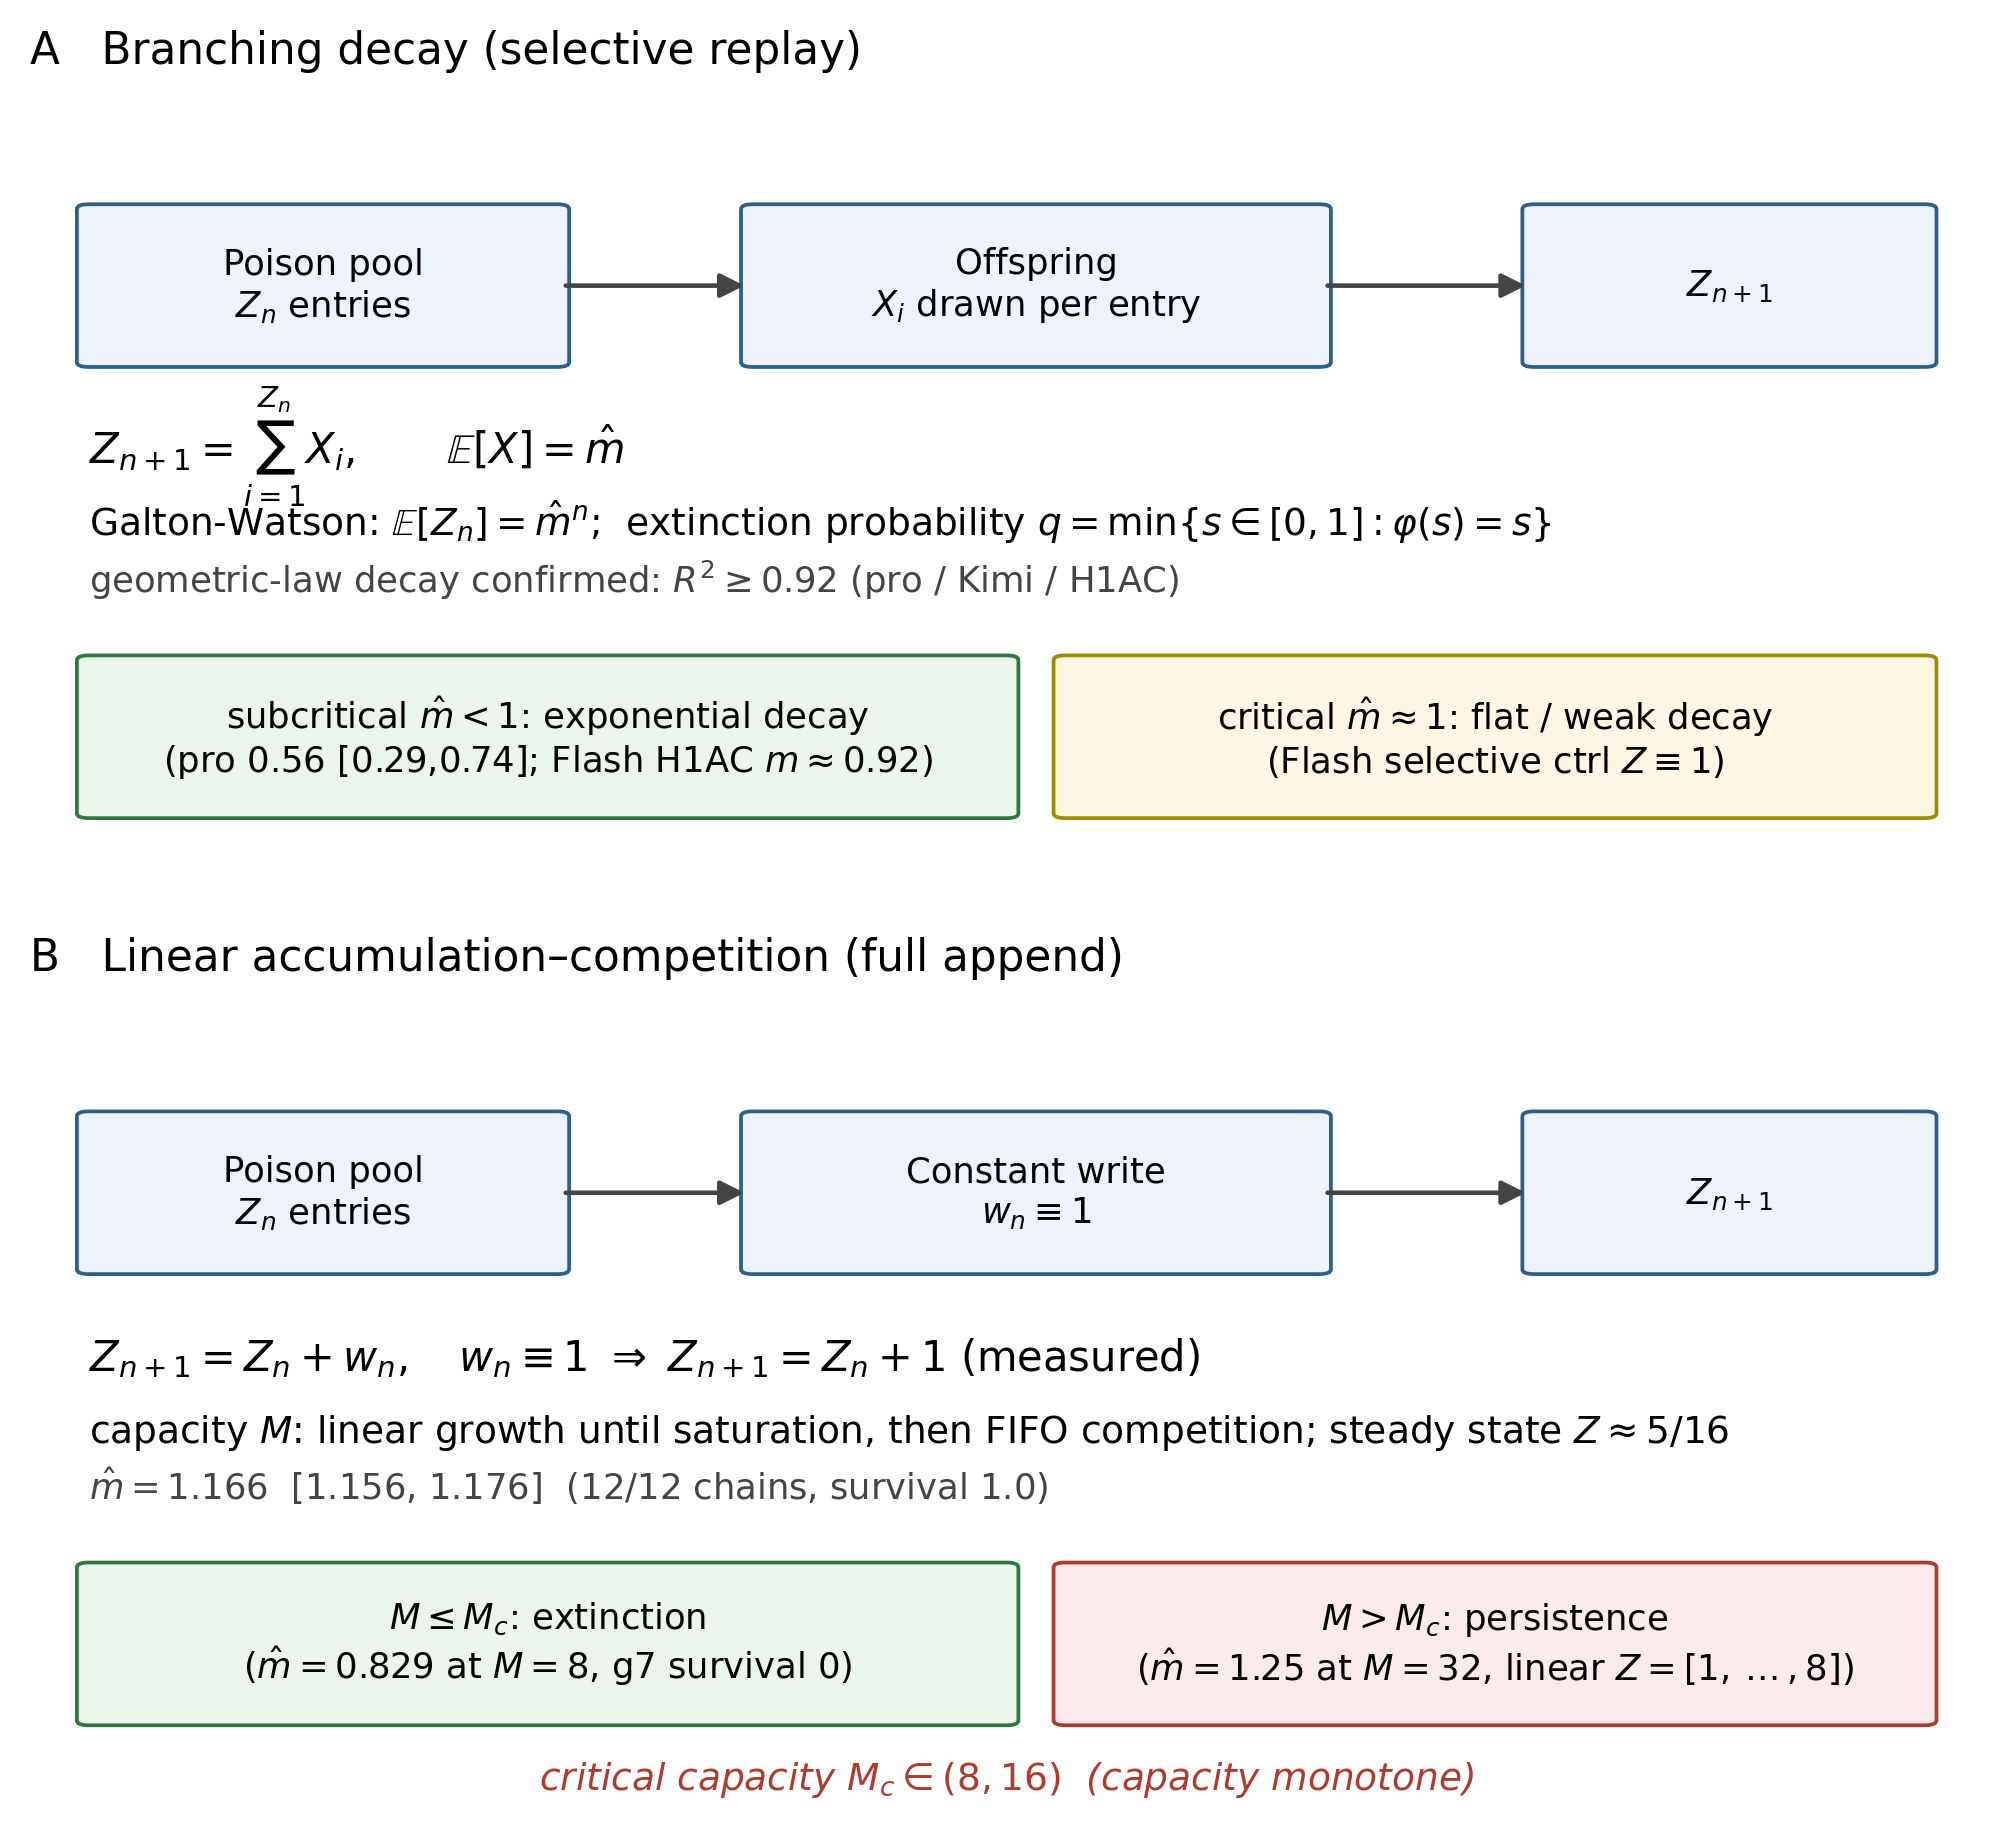
\includegraphics[keepaspectratio,alt={机制示意：分支衰减（选择性转写）与线性累积-容量竞争（全量追加）}]{figures/fig-mechanism.png}}
\caption{机制示意：分支衰减（选择性转写）与线性累积-容量竞争（全量追加）}
\end{figure}

\emph{图 1 两种传播机制：A）选择性转写下的分支衰减（Galton-Watson
分支过程、几何律，灭绝概率=最小不动点）；B）全量追加下的线性累积-容量竞争（每代写入
\(w_n\in\{0,1\}\)、链均 \(E[w_n]=0.917\)，容量 \(M\) 处 FIFO 竞争，临界
\(M_c\in(8,16)\)（低转写态读数））。}（数据：DeepSeek-V4.1-Flash-1017，链均）

\subsection{4 形式化}\label{ux5f62ux5f0fux5316}

\subsection{4.1 模型结构}\label{ux6a21ux578bux7ed3ux6784}

传播模型为\textbf{分支过程}（\texttt{BranchingProcess}
结构，每代一个有限支撑
PMF）：未终审经验的跨代传播中，双盲隔离门禁的选择度 \(\sigma\)
将名义繁殖均值 \(\mu\) 压缩为有效繁殖数

\[m = \mu(1-\sigma) \quad \text{(乘性压缩律)}\]

所有定理以\textbf{条件定理}呈现：结构前提（如
\(m<1\)）为显式假设，``真实系统满足该前提''由 §5--§6
实测支撑，不在形式系统内断言。这一分工即本文采用的三层知识地位结构：\textbf{定理层}（Lean
机检的结构蕴含）、\textbf{经验层}（\(\hat m\)、\(M_c\)、\(\sigma\)
等参数的预注册实测）、\textbf{工程层}（生产判据的部署裁决）；数值与定理互不冒充。\(\sigma\)
的口径与 §3.1 一致（拦截率，写出通过率 \(=1-\sigma\)）；EXP-A
的随机过滤档以放行率 \(r=1-\sigma\) 实现（表 5 标注，§6.5）。

\subsection{4.2 定理链}\label{ux5b9aux7406ux94fe}

本节定理链全部由 Lean 4 机器验证（零
\texttt{sorry}）。形式化源码：\texttt{formal\_proof/IACFormalization}（本仓库
commit \texttt{4825137}；Lean 4，mathlib 版本见
\texttt{lakefile.lean}）。仓库目前\textbf{保持私有}：commit hash
可据此核对文件树与构建记录，完整源码按需向作者索取。

\textbf{T1
期望几何律}（\texttt{expected\_population\_geometric}，归纳证明）：\(E[Z_n]=m^n E[Z_0]\)。

\textbf{T2
亚临界概率灭绝}（\texttt{subcritical\_extinction\_in\_probability}）：由
Markov 不等式与几何衰减，\(m<1\) 时存活概率
\(P(Z_n\ge1)\to0\)。这是隔离晋升门禁有效性的定量核心：门禁把 \(m\) 压到
\(<1\)，长期存活概率
\(P(Z_n\ge1)\to0\)（依概率收敛）------应用侧措辞严格为``存活概率趋向
0''，而非``以概率 1 消亡''。

\textbf{T3
隔离压缩后代}（\texttt{quarantine\_compresses\_offspring}）：\(\sigma\)
越严格，有效繁殖数越小；完全隔离（\(\sigma=1\)）使
\(m=0\)，谱系单代内归零。\textbf{应用条件}：分支性 + 乘性压缩------在
selective 架构下实测满足（几何律 \(R^2=0.958\)）；在 full-append
架构下分支前提不成立，隔离的有效性由实测直接给出（C3-full 12/12，mem 恒
6、\(Z\) 恒 1），机制修正记录在案（§9）。

\textbf{T4 超临界不灭绝}（\texttt{galton\_watson\_non\_extinction} +
\texttt{supercritical\_expectation\_diverges}）：\(m>1\)
时，灭绝概率为生成函数 \(\varphi\) 在 \([0,1]\) 上的\textbf{最小不动点}
\(q=\min\{s\in[0,1]:\varphi(s)=s\}<1\)------以正概率永不灭绝；期望
\(E[Z_n]\to+\infty\)。证明采用初等生成函数不动点分析（单调夹逼 +
多项式截断），避免对 \(\varphi\) 连续性的依赖。

\subsection{4.3
定理-应用映射}\label{ux5b9aux7406-ux5e94ux7528ux6620ux5c04}

{\def\LTcaptype{} % do not increment counter
\begin{longtable}[]{@{}
  >{\raggedright\arraybackslash}p{(\linewidth - 4\tabcolsep) * \real{0.3333}}
  >{\raggedright\arraybackslash}p{(\linewidth - 4\tabcolsep) * \real{0.3333}}
  >{\raggedright\arraybackslash}p{(\linewidth - 4\tabcolsep) * \real{0.3333}}@{}}
\toprule\noalign{}
\begin{minipage}[b]{\linewidth}\raggedright
定理
\end{minipage} & \begin{minipage}[b]{\linewidth}\raggedright
断言
\end{minipage} & \begin{minipage}[b]{\linewidth}\raggedright
应用侧
\end{minipage} \\
\midrule\noalign{}
\endhead
\bottomrule\noalign{}
\endlastfoot
T1 & \(E[Z_n]=m^nE[Z_0]\) & 几何律判据（S-H2/B-H2 的期望侧） \\
T2 & \(m<1 \Rightarrow P(Z_n\ge1)\to0\) & 隔离/随机过滤压灭谱系（C2
存活率 0.062 vs C0 0.750） \\
T3 &
\(\sigma\!\uparrow \Rightarrow m\downarrow\)；\(\sigma=1\Rightarrow m=0\)
& 隔离不变性（S-H4/T-H1/X-H1） \\
T4 & \(m>1 \Rightarrow q<1\)，\(E[Z_n]\to+\infty\) & 机制 A
超临界侧对照；机制 B 的持续累积由实测占据率给出（工程语义） \\
\end{longtable}
}

\subsection{4.5 机制 B
稳态占据率}\label{ux673aux5236-b-ux7a33ux6001ux5360ux636eux7387}

本节命题为普通数学推导，未经 Lean 机器验证。\textbf{命题（机制 B
稳态占据率）}：full-append 架构、FIFO 容量 \(M\)、每代良性写入 \(b\)
条、毒株写入链均
\(\bar w\)（\(0<\bar w\le1\)）时，在''毒株条目在容量内均匀混合''的近似下，稳态毒株占据为

\[Z^* = \frac{M\,\bar w}{b+\bar w}\]

\textbf{证明}：每代写入总量期望 \(b+\bar w\) 条（毒株 \(\bar w\)
条）；FIFO 每代挤出等量最旧条目。若毒株均匀分布于 \(M\)
槽位，则每代被挤出的毒株数期望为
\((b+\bar w)\cdot Z/M\)。稳态要求流入等于流出：\((b+\bar w)\cdot Z^*/M = \bar w\)，即
\(Z^*=M\bar w/(b+\bar w)\)。\(\blacksquare\)

\textbf{实测验证}：C0-full（\(b=2\)、\(\bar w=0.917\)、\(M=16\)）预测
\(Z^*=16\times0.917/2.917=5.03\)，实测稳态 4.917（g5--g7
稳定），相对偏差 2.3\%。

\textbf{限定}：均匀混合为近似------FIFO
下毒株条目位置分布非均匀且存在代际相关性，精确解依赖具体写入序列；本文以该闭式作为机制
B 的\textbf{内生稳态描述量}（取代 GW 参数的机制内生化，§9）。

\subsection{4.6
形式化的边界}\label{ux5f62ux5f0fux5316ux7684ux8fb9ux754c}

机制 A 的 \(\hat m\)、\(M_c\)、\(\sigma\)
的\textbf{数值}为经验/工程层参数，不入形式化接口（机制 B 无 GW 语义的
\(\hat m\)，其传播比估计见 §6.1
表注）；形式化保证的是\textbf{结构蕴含}（若前提成立则结论必真），数值由预注册实测估计。这一分工避免了两类错误：把经验常数当定理、把定理当经验常数。

\subsection{5 实验设置}\label{ux5b9eux9a8cux8bbeux7f6e}

\subsection{5.1 预注册原则}\label{ux9884ux6ce8ux518cux539fux5219}

全部判据先于实验固定（假说清单见 §3.5）：显著性门槛（\(p<0.05\)
置换/单侧）、判读单位（链均 vs 池化，见
5.5）、方向性命题一律预先声明。实验计划文档随判读产物存档（\texttt{EXPERIMENT\_PLAN\_AXIOM4\_SUPERCRITICAL.md}、\texttt{EXPERIMENT\_PLAN\_AXIOM4\_H1AC\_BOOST.md}），任何口径修订在
§11 记录在案（如 H1AC 池化口径失效）。

\subsection{5.2 模型档}\label{ux6a21ux578bux6863}

{\def\LTcaptype{} % do not increment counter
\begin{longtable}[]{@{}
  >{\raggedright\arraybackslash}p{(\linewidth - 4\tabcolsep) * \real{0.3333}}
  >{\raggedright\arraybackslash}p{(\linewidth - 4\tabcolsep) * \real{0.3333}}
  >{\raggedright\arraybackslash}p{(\linewidth - 4\tabcolsep) * \real{0.3333}}@{}}
\toprule\noalign{}
\begin{minipage}[b]{\linewidth}\raggedright
档
\end{minipage} & \begin{minipage}[b]{\linewidth}\raggedright
模型
\end{minipage} & \begin{minipage}[b]{\linewidth}\raggedright
用途
\end{minipage} \\
\midrule\noalign{}
\endhead
\bottomrule\noalign{}
\endlastfoot
主实验 & \textbf{DeepSeek-V4-Pro-0813}（简称 Pro；采样温度 temperature
0.7） & selective 协议，4 条件 × 12 会话 × 6 代 = 288 会话 \\
跨模型 & Kimi \texttt{kimi-for-coding} + 同 Pro 协议 & X-H1/X-H4，288
会话 \\
SUPERCRITICAL & \textbf{DeepSeek-V4.1-Flash-1017}（简称 Flash） &
full-append/容量档/selective 对照（与预注册模型档的偏离已在计划 §10
记录） \\
H1AC & 同 Flash & 160 链双毒株大样本 \\
COMPLEMENT-EXP & 同 Flash & 隔离代价 σ 扫描（EXP-A 240）/ \(b\times M\)
容量曲面（EXP-B 144）/ selective 扩样 n=12（EXP-C） \\
\end{longtable}
}

\subsection{5.3 传播协议}\label{ux4f20ux64adux534fux8bae}

\begin{itemize}
\tightlist
\item
  \textbf{毒株规范注入}：第 0 代注入 1
  条携带谱系标记（P1/P2）的种子经验；逐代转写（selective：仅被判定相关者转写；full-append：全量追加）；
\item
  \textbf{谱系追踪}：每条记忆条目携带 lineage 标记，\(Z_n\)=第 \(n\)
  代毒株谱系条目数（判读单位）；
\item
  \textbf{双盲过滤（DRAFT\_SUSPECT）}：标记门条件（C1）对疑似条目打标但不阻断；隔离门禁（C3/C2）物理阻断未终审条目（即未通过五重物理判据与独立审查终审的条目，定义见
  §2.3）。
\end{itemize}

\subsection{5.4 条件矩阵}\label{ux6761ux4ef6ux77e9ux9635}

\begin{itemize}
\tightlist
\item
  \textbf{selective}：C0（无门禁）/ C1（标记门）/ C2（随机过滤
  \(\sigma=0.5\)）/ C3（隔离 \(\sigma=1\)）；
\item
  \textbf{full-append}：C0-full / C1-full / C3-full（各 12 会话 × 8
  代）；容量档 \(M=8\) / \(M=32\)（各 6 会话 × 8 代）；selective 对照（2
  会话 × 6 代）；
\item
  \textbf{H1AC（Flash 双毒株）}：C0（48）/ C1（48）/ C2（64），6 代。
\end{itemize}

\textbf{合计 846 条智能体会话链}（= 主实验 48 + 跨模型 48 + 跨任务族 144
+ SUPERCRITICAL 50 + H1AC 160 + COMPLEMENT-EXP 396；会话-代单元口径合计
5,448 = 288 + 288 + 864 + 384 + 960 + 2,664；selective 对照 2 链 × 6 代
= 12 单元，不在合计内、另计）。其中 SUPERCRITICAL 50 链 = 3 条件 × 12 链
× 8 代（C0/C1/C3-full）+ 敏感性 2 档 × 6 链 × 8 代（W=8/32）；H1AC 160
链 = C0 48 + C1 48 + C2 64，× 6 代；跨任务族 144 链 × 6
代；COMPLEMENT-EXP 396 链 = EXP-A 240（σ 扫描 5 档 × 48 链，× 6 代）+
EXP-B 144（\(b\times M\) 曲面 24 档 × 6 链，× 8 代）+ EXP-C
12（selective 扩样，× 6 代），判读脚本 \texttt{kimi\_boost\_judge.py}
可复算。\textbf{时间线}：DeepSeek-V4.1-Flash-1017 于 2026-10-17
发布，SUPERCRITICAL 与 H1AC 全部实验于发布后 5
日内（2026-10-22）完成执行与判读，COMPLEMENT-EXP 三实验于发布后 6
日内（2026-10-23）完成执行与判读（各批次运行时间戳见附录 A）。

\subsection{5.5 判读口径}\label{ux5224ux8bfbux53e3ux5f84}

\begin{itemize}
\tightlist
\item
  bootstrap CI（\(10^4\) 重采样）估计 \(\hat m\) 及比值
  CI；符号翻转配对置换（\(10^4\)）检验标记门配对差；
\item
  \textbf{链均 vs 池化}：传播实验的判读单位取链均（per-parent 池化在 C2
  下因幸存者偏差失效------末代存活率仅 6\%，池化比值 1.017
  无意义；已在计划 §10 记录并改用链均）；
\item
  几何律复验：log-linear 拟合 \(R^2\)；
\item
  \textbf{功效}（Pro 档标记门）：配对差 \(d=0.167\)、\(sd=0.432\)、C1/C0
  比值 0.529 → 当前 \(n=12\) 功效仅 0.38，达 0.8 需
  \(n\approx48\)（\texttt{e\_power\_markgate.py/.json}）------H1AC 档以
  48 配对补齐该缺口。
\end{itemize}

\subsection{5.6 可复现性}\label{ux53efux590dux73b0ux6027}

\begin{itemize}
\tightlist
\item
  判读脚本：\texttt{e\_supercritical\_judge.py}/\texttt{judge2.py}/\texttt{sh3.py}、\texttt{e\_cross\_task\_judge.py}、\texttt{e\_h1ac\_judge.py}（全部入
  git）；
\item
  原始会话：\texttt{axiom4\_results\_*.json}（SUPERCRITICAL/H1AC/跨模型/跨任务族全套入
  git）；
\item
  环境：模型档固定、采样温度 0.7、采样参数随会话归档。
\end{itemize}

\subsection{6 结果}\label{ux7ed3ux679c}

\subsection{6.1 机制与容量}\label{ux673aux5236ux4e0eux5bb9ux91cf}

本节数据来自 SUPERCRITICAL 档（Flash，full-append 转写）。\textbf{S-H1
机制 B 判据 ✅（GW 表述已失效）}：S-H1 的 GW 表述（\(\hat m>1\) 且 CI
下限 \(>1\)）随 S-H3
证伪而失效------对确定性线性累积过程，任何增长型统计量必
\(>1\)，该判据在机制 B 下设计上不可能失败（§9）。机制 B
的内生判据为：\textbf{持续累积}（未饱和段线性增长，饱和后稳态 \(5/16\)
维持 3 代）+ \textbf{存活率 1.0}，二者均满足。Z 轨迹
\([1,2,2.917,3.917,3.917,4.917,4.917,4.917]\)：g0--g3 线性累积，g4
触及容量（mem 6→16），g5--g7 FIFO 稳态 4.917。跨机制对比的传播比
\(\hat m^\dagger=1.166\)（{[}1.156,1.176{]}；估计器
\(\hat m=\sum Z_{n+1}/\sum Z_n\)，§3.1；GW``每亲繁殖数''语义仅机制 A
有效）。

\textbf{S-H2 存活率 ✅}：g7 存活率 1.0（12/12 链无灭绝）。

\textbf{S-H3 GW 匹配 ✗（被机制证据证伪）}：逐代 offspring
核对------每代新写 P1 为 0 或 1（\(w_n\in\{0,1\}\)，PMF={[}0,1{]}，链均
\(E[w_n]=0.917\)，11/12 链每代恒 1、约 1/12
链存在某代未写），且写入不依赖
\(Z_n\)------分支过程要求的``后代数依赖亲代种群''不成立。机制
B（线性累积-容量竞争）取代 GW 匹配；\textbf{修订叙事见 §9}。

\textbf{S-H4 隔离不变性 ✅}：C3-full 12/12 链 mem 恒 6、\(Z\) 恒
1------隔离在 full-append 架构下同样截断传播（即使分支前提不成立）。

\textbf{容量控制参量}：\(M=8\) 时传播比
\(\hat m^\dagger=0.829\)（\([0.739,0.875]\)），g7 存活率
0（灭绝）；\(M=32\) 时 \(\hat m^\dagger=1.25\)（退化 CI，6
链全同），\(Z=[1,\dots,8]\) 线性增长未饱和。\textbf{临界
\(M_c\in(8,16)\)}（本协议档，\(b=3\)，\textbf{低转写态读数}------探针门控重扫实测高转写态下
\(W{=}8\) 存活 0.75、\(M_c\in(4,8)\)，§6.5），容量单调性成立；补充实验
EXP-B 证实 \(M_c\) 是 \((b,M)\) 联合函数（§6.5）。

\textbf{selective 对照（Flash）}：主实验 2 链 \(Z\) 恒 1、记忆收缩至
3（\(\hat m=1.0\) 临界边界；H1AC 大样本 48 链 \(m\approx0.92\)
支持弱亚临界）------同一模型档下与 C0-full
构成架构分叉（§3.4）。\textbf{补充实验
EXP-C（n=12，2026-10-23）}：\(\hat m=0.966\)（boot95 CI
\([0.911,1.000]\)，含 1）、几何律 \(R^2=0.833\)、\(Z\) 均值
\([1,1,1,0.917,0.917,0.833]\)、最终代存活 0.83------\textbf{与
C0-full（\(\hat m=1.166\)，CI \([1.156,1.176]\)）两 CI
完全分离}，selective 亚临界/临界保持在 n=12 下统计成立，架构分叉承重墙由
2 链扩至 12 链（C-H1/C-H2 ✅）。

\subsection{6.2
标记门与乘性律}\label{ux6807ux8bb0ux95e8ux4e0eux4e58ux6027ux5f8b}

本节数据来自 H1AC 档（Flash，160 链）。\textbf{B-H1a 标记门压缩
✗}：配对（C0 vs C1，48 对）差值
\(\bar d=+0.020\)（均值被少数大差对拉动；正差仅
15/48，配对层面多数反预期）、符号翻转置换 \(p=0.69\)------\textbf{Flash
档零压缩}。三档证据分层：Pro
主实验为\textbf{功效不足下的大效应不显著}（\(p=0.15\)，C1/C0 比值
0.529、压缩 47\%，功效 0.38，不可判读为零压缩）→ SUPERCRITICAL C1-full
12/12 逐代同轨（full-append 写路径结构绕过模型判断，非软信号独立证据）→
H1AC 大样本配对确证零压缩。功效侧：H1AC 的 \(n=48\) 已达 Pro
档功效分析所需样本（功效 0.848），排除''功效不足''解释。

\textbf{B-H1c 乘性压缩律（部分）}：链均写入率比
\(\hat r=\mu_{C2}/\mu_{C0}=0.422/0.905=\boldsymbol{0.466}\in[0.35,0.65]\)（乘性预测
0.5 吻合）；bootstrap CI \([0.333,0.602]\)------下界微出目标带
0.017。判据定义（点估计+CI 双判据）：点估计 ✅、CI ⚠️。存活率佐证：C2
末代 0.062 vs C0 0.750------随机过滤真实压低传播。

\textbf{B-H2 几何律复验 ✅}：C0/C1 的 \(\log Z\) 对代际线性拟合
\(R^2=0.923\)、\(m\approx0.92\)（Flash selective 临界/弱亚临界，与主实验
\(R^2=0.958\) 一致）。

\textbf{P2 事件倍增未达成}：\(\mu_{P2}\approx0.001\)（250 vs 1
条）------双毒株设计的第二事件通道未被模型采纳（记录在案，§11）。

\subsection{6.3 跨模型}\label{ux8de8ux6a21ux578b}

跨模型实验共 288 会话（selective 转写）。\textbf{X-H1/X-H4 ✅}：无门禁下
\(\hat m\) 模型特定（Pro 0.560 {[}0.294,0.735{]}、Kimi 0.983
{[}0.944,1.000{]}、Flash 1.0 临界；转写衰减倾向异质，全名见
§5.2），但隔离保证跨模型成立（24/24 链
\(Z_1=0\)）------防御不依赖模型行为。判读汇总见 §6.6 表 3。

\subsection{6.4 跨任务族}\label{ux8de8ux4efbux52a1ux65cf}

跨任务族实验共 144 链（selective 转写）。隔离 48/48 链灭绝（T-H1
✅）；毒株传播受任务族调节（T-H4 配对 \(p=0.026\) ✅）；无门禁
\(\hat m\) 为模型-任务-位点联合参数（跨任务族区间
\([0.29,1.00]\)）------\textbf{跨族不可迁移是实测结论而非缺陷}（§10）。

\subsection{6.5
隔离代价与容量曲面}\label{ux9694ux79bbux4ee3ux4ef7ux4e0eux5bb9ux91cfux66f2ux9762}

本节为补充实验（Flash，共 396 链）。\textbf{EXP-A 隔离代价（σ 扫描 × 48
链，full-append W=16，6 代；σ 语义见表 5 标注：A50/A75/A90/A25/A10
档放行率 \(r=0.5/0.75/0.9/0.25/0.1\)，等价拦截率
\(\sigma_{\rm eff}=0.5/0.25/0.1/0.75/0.9\)；A100 隔离档
\(\sigma_{\rm eff}=1\)）}：A100（硬隔离）\(Z\) 最终代恒
1、记忆不增长（mem\_growth=0.00，n=48）------\textbf{硬隔离阻断一切未终审写入，累积传播零出现（A-H1
✅，按''无累积传播''口径，同 §9.3 S-H4
先例）}；\(\sigma_{\rm eff}=0.1\)（A90）抑制不足（\(Z_f=4.60\)，传播仍在）。\textbf{甜点补测（2026-10-23，A25/A10
两档各 48 链，KIMI 三轮 N3
作业）}：A25（\(\sigma_{\rm eff}=0.75\)）\(Z_f=2.00\)、\textbf{存活率
1.00}、效用保留
1.12；A10（\(\sigma_{\rm eff}=0.9\)）\(Z_f=1.60\)、\textbf{存活率
1.00}、效用保留 0.96------\textbf{全谱
\(\sigma_{\rm eff}\in\{0.1,0.25,0.5,0.75,0.9\}\) 无一档存活率
\textless0.1（全部 1.00），A-H4
判据：无甜点}；拦截率越高毒株累积越低（\(Z_f\)
单调下降），但\textbf{只要放行率非零，毒株就不灭绝}（线性累积 \(w_n\)
均值仍正），仅硬隔离（\(\sigma_{\rm eff}=1\)）根除。代价侧：良性通过率实测
0.488/0.754/0.908/0.262/0.094/0.000 = 放行率
\(r\)（\(=1-\sigma_{\rm eff}\)，无差别随机过滤，A-H2
✅），隔离档的记忆效用保留 0.88（相对 C0 良性存量
-12\%，全部为新经验增量损失，种子基线 6
条无损）。\textbf{容量竞争的意外发现}：拦截率中档（\(\sigma_{\rm eff}=0.5/0.25/0.1\)）的良性存量\textbf{反高于无门禁
C0}（效用保留 1.33/1.31/1.19）------过滤门压制毒株后，良性条目在 FIFO
中获得更大份额，误拦（\(\sigma_{\rm eff}\)）被份额补偿抵消。\textbf{二维代价-收益结论（已测全谱
\(\sigma_{\rm eff}\in\{0.1,0.25,0.5,0.75,0.9,1.0\}\)）：不存在同时抑制毒株且保留新经验增量的档------硬隔离（\(\sigma_{\rm eff}=1\)）收益达标但
-12\% 增量，\(\sigma_{\rm eff}<1\) 保留增量但毒株超临界（存活率
1.00）}。

\textbf{EXP-B 容量曲面（\(b\times M\)，24 档 × 6 链，8 代）}：临界容量
\(W_c(b)\) 随良性写入率 \(b\) 上移------\(b=1/2\) 时
\(W_c\le4\)，\(b=3\) 时 \(W_c\in(4,8)\)，\(b=5\) 时
\(W_c\in(8,12)\)（漂移跨度 ≥2 档，B-H2 ✅）→ \textbf{\(M_c\) 是
\((b,M)\) 联合函数}（§6.1 的''当前协议下 \(M_c\in(8,16)\)``为 \(b=3\)
档实例）。机制解读：良性写入与毒株竞争 FIFO 容量------\(b=5, W=4\)
时毒株灭绝（\(Z\) 末代 0、\(\hat m=0.143\)），\textbf{高 \(b\) + 低
\(M\) 是容量竞争的天然亚临界}。非单调异常记录在案：\(b=2, W=4\) 存活率
1.00（高于 \(b=1\) 的 0.50），6 链强随机性下保留不解释。

\textbf{\(W{=}8\) 分裂归因（KIMI 三轮作业 2
重跑对照，2026-10-23）}：原分裂=主协议（10-22）\(W{=}8\) 6/6 全灭 vs
EXP-B（10-23）\(b{=}3,W{=}8\) 12 链存活 0.92。静态逐行审计两脚本
\(b{=}3\) 档：提示文本、FIFO
实现、门禁（无）、任务序列、种子记忆逐字一致------diff
为空。同日重跑（同一脚本、同协议、同 rep 序号、scnet-flash）：

{\def\LTcaptype{} % do not increment counter
\begin{longtable}[]{@{}
  >{\raggedright\arraybackslash}p{(\linewidth - 10\tabcolsep) * \real{0.1429}}
  >{\raggedright\arraybackslash}p{(\linewidth - 10\tabcolsep) * \real{0.1429}}
  >{\centering\arraybackslash}p{(\linewidth - 10\tabcolsep) * \real{0.1786}}
  >{\centering\arraybackslash}p{(\linewidth - 10\tabcolsep) * \real{0.1786}}
  >{\centering\arraybackslash}p{(\linewidth - 10\tabcolsep) * \real{0.1786}}
  >{\centering\arraybackslash}p{(\linewidth - 10\tabcolsep) * \real{0.1786}}@{}}
\toprule\noalign{}
\begin{minipage}[b]{\linewidth}\raggedright
批次
\end{minipage} & \begin{minipage}[b]{\linewidth}\raggedright
日期
\end{minipage} & \begin{minipage}[b]{\linewidth}\centering
\(n\)
\end{minipage} & \begin{minipage}[b]{\linewidth}\centering
存活率
\end{minipage} & \begin{minipage}[b]{\linewidth}\centering
毒株写入/链（8 代合计）
\end{minipage} & \begin{minipage}[b]{\linewidth}\centering
Fisher \(p\)（vs 10-22 主协议）
\end{minipage} \\
\midrule\noalign{}
\endhead
\bottomrule\noalign{}
\endlastfoot
主协议 \(W{=}8\) 原批 & 10-22 & 6 & \textbf{0.000} & 2.00 & --- \\
主协议 \(W{=}8\) 重跑 & 10-23 & 12 & 0.583 & 5.33 & \textbf{0.038} \\
EXP-B \(b{=}3\|W8\) 原批 & 10-23 & 12 & 0.917 & 6.75 & 0.0004 \\
EXP-B \(b{=}3\|W8\) 重跑 & 10-23 & 12 & 0.583 & 5.00 & \textbf{0.038} \\
\end{longtable}
}

\textbf{归因}：存活率与毒株转写率完全单调对应（avg\_pw 2.00 → 存活
0；5.0--6.75 → 存活 0.58--0.92），毒株转写率是 \(W{=}8\)
存活的唯一驱动因子；同日两脚本（主协议重跑 vs EXP-B
原批/重跑）无显著差异（Fisher \(p{=}0.155\)），10-22
主协议批次显著偏低（vs 全部 10-23 数据
\(n{=}36\)，\(p{=}0.0024\)）。\textbf{``\(W{=}8\)
跨协议分裂''不成立------分裂的真实来源是 DeepSeek-V4.1-Flash-1017
毒株转写行为的亚小时级状态切换}（10-22 15:30 C0-full 高转写态 0.917/代
vs 16:02 \(W{=}8\) 原批低转写态 0.25/代，同一日历日内约 32
分钟翻转，附录 A 时间戳；同日双脚本重跑无差异 \(p{=}0.155\)
排除协议因素），主协议 \(W{=}8\) 6/6
全灭是\textbf{低转写态}下的读数而非结构性临界；\textbf{\(M_c\)
绝对读数标记为状态敏感}（低转写态下 \(M_c\in(8,16)\)、\(W{=}8\)
灭绝；高转写态下 \(W{=}8\) 存活过半、\(M_c<8\)------\(M_c=(b,M,\)
毒株转写状态\()\) 条件量；同批内相对比较------EXP-B 24
档曲面、SUPERCRITICAL 档内------不受影响）。漂移区间已量化（四批毒株写入
2.00--6.75/链、存活率
0--0.92，§11.4）；残余开放项收窄为毒株转写率的\textbf{批次预测模型未建立}（§11.4）。

\textbf{状态条件量实测（探针门控重扫，2026-10-23
19:0x）}：按预注册判据（计划 §1.2e 预先固定：高转写态下 \(W{=}8\) 存活率
\(\ge0.5\) ⟹ \(M_c\) 改述为状态条件量），先以 2
条状态探针判定当前毒株转写态（18:48--18:51，C0-full W16 6
代，\textbf{\(p_{\rm probe}{=}1.000\)
高转写态}），随后在同一协议（\texttt{axiom4\_memory\_propagation.py}
full\_append C0 6 代，与主实验逐字一致）下重跑 \(W\in\{4,8,12\}\) 各 12
链：

{\def\LTcaptype{} % do not increment counter
\begin{longtable}[]{@{}
  >{\raggedright\arraybackslash}p{(\linewidth - 8\tabcolsep) * \real{0.1667}}
  >{\centering\arraybackslash}p{(\linewidth - 8\tabcolsep) * \real{0.2083}}
  >{\centering\arraybackslash}p{(\linewidth - 8\tabcolsep) * \real{0.2083}}
  >{\centering\arraybackslash}p{(\linewidth - 8\tabcolsep) * \real{0.2083}}
  >{\centering\arraybackslash}p{(\linewidth - 8\tabcolsep) * \real{0.2083}}@{}}
\toprule\noalign{}
\begin{minipage}[b]{\linewidth}\raggedright
档（高转写态）
\end{minipage} & \begin{minipage}[b]{\linewidth}\centering
\(n\)
\end{minipage} & \begin{minipage}[b]{\linewidth}\centering
存活率
\end{minipage} & \begin{minipage}[b]{\linewidth}\centering
毒株写入/链
\end{minipage} & \begin{minipage}[b]{\linewidth}\centering
vs 低态原批
\end{minipage} \\
\midrule\noalign{}
\endhead
\bottomrule\noalign{}
\endlastfoot
\(W{=}4\) & 12 & 0.417（5/12） & 3.50 & 低态无对照档 \\
\(W{=}8\) & 12 & \textbf{0.750（9/12）} & 4.42 & 低态
0.000（0/6），Fisher 双侧 \(p{=}0.009\) \\
\(W{=}12\) & 12 & \textbf{1.000（12/12）} & 6.00 & 低态
1.000（SUPERCRITICAL W16 持续） \\
\end{longtable}
}

\textbf{判据满足}：高转写态下 \(W{=}8\) 存活率 0.750
\(\ge0.5\)------\textbf{\(M_c\) 状态条件量实证成立}：高转写态
\(M_c\in(4,8)\)（\(W{=}4\) 0.417 \textless0.5、\(W{=}8\) 0.750
≥0.5），低转写态 \(M_c\in(8,16)\)（\(W{=}8\) 灭绝）。同一记忆窗口
\(W{=}8\)
在低转写态下灭绝、高转写态下存活过半------\textbf{``缩小记忆窗口不能可靠防住投毒''由双态对照直接实证}；高态
\(W{=}8\) 存活 0.750 与 10-23
同日重跑批次（0.583--0.917）同量级，批内一致性良好（数据与判读：\texttt{\_mc\_state\_rescan\_W\{4,8,12\}\_\{s1,s2\}.json}、\texttt{\_mc\_state\_rescan\_judge.txt}）。

\subsection{6.6 工程侧}\label{ux5de5ux7a0bux4fa7}

本节为生产现场的关联实证。生产现场闭环实验（智能体自主提交 →
五重物理判据晋升/拦截 → 审计归档）：18 份报告晋升 14、拦截 4；晋升比例
1.00、错误拦截 1.00、泄漏 0。\textbf{口径说明}：晋升比例 1.00 = 14/14
晋升报告经复核均为正确经验；错误拦截 1.00 = 4/4
拦截报告均为错误经验（拦截正确率）；泄漏 0 =
晋升集不含错误经验。该表为生产现场关联实证（\(n=18\)），代价侧（良性误拦率）的正式估计需
§6.5
以外的更大样本（开放项，§11.4）；工程闭环与理论通道的连接亦为开放项，不构成跨通道因果声称。

\begin{center}\rule{0.5\linewidth}{0.5pt}\end{center}

\subsection{6.7 正式判读表}\label{ux6b63ux5f0fux5224ux8bfbux8868}

以下表格数值直接来自判读脚本输出的
JSON（数据直出，无手工转录）。\textbf{表 1：机制与容量（SUPERCRITICAL
档，Flash，full-append，链均）}

{\def\LTcaptype{} % do not increment counter
\begin{longtable}[]{@{}
  >{\raggedright\arraybackslash}p{(\linewidth - 12\tabcolsep) * \real{0.1212}}
  >{\centering\arraybackslash}p{(\linewidth - 12\tabcolsep) * \real{0.1515}}
  >{\centering\arraybackslash}p{(\linewidth - 12\tabcolsep) * \real{0.1515}}
  >{\raggedright\arraybackslash}p{(\linewidth - 12\tabcolsep) * \real{0.1212}}
  >{\centering\arraybackslash}p{(\linewidth - 12\tabcolsep) * \real{0.1515}}
  >{\centering\arraybackslash}p{(\linewidth - 12\tabcolsep) * \real{0.1515}}
  >{\centering\arraybackslash}p{(\linewidth - 12\tabcolsep) * \real{0.1515}}@{}}
\toprule\noalign{}
\begin{minipage}[b]{\linewidth}\raggedright
条件
\end{minipage} & \begin{minipage}[b]{\linewidth}\centering
容量 \(M\)
\end{minipage} & \begin{minipage}[b]{\linewidth}\centering
\(n\)
\end{minipage} & \begin{minipage}[b]{\linewidth}\raggedright
传播比 \(\hat m^\dagger\)（boot95 CI）
\end{minipage} & \begin{minipage}[b]{\linewidth}\centering
Z 末代（g7）
\end{minipage} & \begin{minipage}[b]{\linewidth}\centering
存活率 g7
\end{minipage} & \begin{minipage}[b]{\linewidth}\centering
判据
\end{minipage} \\
\midrule\noalign{}
\endhead
\bottomrule\noalign{}
\endlastfoot
selective ctrl & 16 & 12（EXP-C 扩样） & 0.966（{[}0.911,1.000{]}） &
1.0 & 1.0 & 临界边界（弱亚临界） \\
C0-full & 16 & 12 & \textbf{1.166}（{[}1.156,1.176{]}） & 4.917（稳态
5/16） & 1.0 & \textbf{S-H1 ✅ S-H2 ✅} \\
C1-full & 16 & 12 & 1.165（{[}1.163,1.167{]}） & 4.917 & 1.0 & 与 C0
逐代同轨（≤0.083） \\
C3-full & 16 & 12 & 1.0（{[}1.0,1.0{]}） & 1.0 & 1.0 & \textbf{S-H4
✅}（mem 恒 6） \\
W=8 & 8 & 6 & 0.829（{[}0.739,0.875{]}） & 0.0 & 0.0 &
\textbf{灭绝}（\(M\le M_c\)，低转写态读数） \\
W=32 & 32 & 6 & 1.25（退化 CI） & 8.0 & 1.0 &
线性增长未饱和（\(M>M_c\)） \\
\end{longtable}
}

临界容量（本协议档，\(b=3\)，\textbf{低转写态读数}）：\(M_c\in(8,16)\)，容量单调性成立（\texttt{capacity\_monotone=True}）；EXP-B
实测 \(M_c\) 为 \((b,M)\) 联合函数（批内曲面，§6.5），\textbf{跨批层面
\(M_c=(b,M,\) 毒株转写状态\()\) 条件量}（高态
\(M_c\in(4,8)\)，§6.5）；跨实验格点核对与协议差异见
§6.5/§3.3。\(\dagger\)：\(\hat m=\sum_n Z_{n+1}/\sum_n Z_n\)（跨代加权平均，源码
\texttt{e\_supercritical\_judge2.py}，可公开复算）；GW''每亲繁殖数''语义仅对机制
A（selective）有效，机制 B 的判定使用占据率与存活率。\(\hat m^\dagger\)
对饱和段敏感（稳态段增量 0 摊薄分子），跨实验比较须同代长。C0/C1 的
\(\hat m^\dagger\)
差异（0.001）为近确定性数据的链间微差，无统计意义，不作为标记门效应的判据。

\textbf{表 2：标记门与乘性律（H1AC 档，Flash，160 链，链均）}

{\def\LTcaptype{} % do not increment counter
\begin{longtable}[]{@{}
  >{\raggedright\arraybackslash}p{(\linewidth - 8\tabcolsep) * \real{0.1905}}
  >{\raggedright\arraybackslash}p{(\linewidth - 8\tabcolsep) * \real{0.1905}}
  >{\raggedright\arraybackslash}p{(\linewidth - 8\tabcolsep) * \real{0.1905}}
  >{\raggedright\arraybackslash}p{(\linewidth - 8\tabcolsep) * \real{0.1905}}
  >{\centering\arraybackslash}p{(\linewidth - 8\tabcolsep) * \real{0.2381}}@{}}
\toprule\noalign{}
\begin{minipage}[b]{\linewidth}\raggedright
假说
\end{minipage} & \begin{minipage}[b]{\linewidth}\raggedright
判读量
\end{minipage} & \begin{minipage}[b]{\linewidth}\raggedright
数值
\end{minipage} & \begin{minipage}[b]{\linewidth}\raggedright
判据
\end{minipage} & \begin{minipage}[b]{\linewidth}\centering
结论
\end{minipage} \\
\midrule\noalign{}
\endhead
\bottomrule\noalign{}
\endlastfoot
B-H1a & 配对差 \(\bar d\)（C0−C1） & +0.020；正差
15/48；\(p=0.69\)（符号翻转 10⁴） & \(p<0.05\) & \textbf{✗ Flash
大样本零压缩}（Pro 档 47\% 不显著） \\
B-H1c & 链均写入率比 \(\hat r=\mu_{C2}/\mu_{C0}\) & 0.422/0.905 =
\textbf{0.466}；CI {[}0.333,0.602{]} & 点∈{[}0.35,0.65{]} 且 CI 全落入 &
⚠️ 点 ✅ CI 下界微出（0.017） \\
B-H2 & log-linear \(R^2\) & \textbf{0.923}；slope
−0.086（\(m\approx0.92\)） & \(R^2\ge0.8\) & \textbf{✅} \\
--- & 存活率末代 & C0=0.750 / C1=0.729 / \textbf{C2=0.062} & 佐证 &
随机过滤真实有效 \\
\end{longtable}
}

\textbf{表 3：跨模型（288 会话，selective；隔离 24/24 链 \(Z_1=0\)）}

{\def\LTcaptype{} % do not increment counter
\begin{longtable}[]{@{}
  >{\raggedright\arraybackslash}p{(\linewidth - 6\tabcolsep) * \real{0.2222}}
  >{\raggedright\arraybackslash}p{(\linewidth - 6\tabcolsep) * \real{0.2222}}
  >{\centering\arraybackslash}p{(\linewidth - 6\tabcolsep) * \real{0.2778}}
  >{\centering\arraybackslash}p{(\linewidth - 6\tabcolsep) * \real{0.2778}}@{}}
\toprule\noalign{}
\begin{minipage}[b]{\linewidth}\raggedright
模型
\end{minipage} & \begin{minipage}[b]{\linewidth}\raggedright
\(\hat m\)（boot95 CI）
\end{minipage} & \begin{minipage}[b]{\linewidth}\centering
隔离保证
\end{minipage} & \begin{minipage}[b]{\linewidth}\centering
判据
\end{minipage} \\
\midrule\noalign{}
\endhead
\bottomrule\noalign{}
\endlastfoot
DeepSeek-V4-Pro-0813（Pro） & 0.560（{[}0.294,0.735{]}） & ✅ &
\textbf{X-H1/X-H4 ✅} \\
Kimi & 0.983（{[}0.944,1.000{]}） & ✅ & 同上 \\
DeepSeek-V4.1-Flash-1017（Flash，selective 对照） &
0.966（{[}0.911,1.000{]}） & ✅ & 同上（EXP-C n=12 扩样） \\
\end{longtable}
}

\textbf{表 4：跨任务族（144 链，selective）}

{\def\LTcaptype{} % do not increment counter
\begin{longtable}[]{@{}
  >{\raggedright\arraybackslash}p{(\linewidth - 4\tabcolsep) * \real{0.3077}}
  >{\raggedright\arraybackslash}p{(\linewidth - 4\tabcolsep) * \real{0.3077}}
  >{\centering\arraybackslash}p{(\linewidth - 4\tabcolsep) * \real{0.3846}}@{}}
\toprule\noalign{}
\begin{minipage}[b]{\linewidth}\raggedright
判据
\end{minipage} & \begin{minipage}[b]{\linewidth}\raggedright
数值
\end{minipage} & \begin{minipage}[b]{\linewidth}\centering
结论
\end{minipage} \\
\midrule\noalign{}
\endhead
\bottomrule\noalign{}
\endlastfoot
T-H1 隔离 48/48 链灭绝 & 48/48 & ✅ \\
T-H4 毒株传播受任务族调节 & 配对 \(p=0.026\) & ✅ \\
无门禁 \(\hat m\) 区间 & {[}0.29, 1.00{]}（模型-任务-位点联合参数） &
跨族不可迁移 \\
\end{longtable}
}

\textbf{表 5：隔离代价（EXP-A，Flash，σ 扫描 × 48 链，full-append
W=16）}

\begin{quote}
标注说明：A50/A75/A90/A25/A10 档以\textbf{随机放行率 \(r\)}
实现（条目以概率 \(r\) 通过门禁），等价拦截率
\(\sigma_{\rm eff}=1-r\)（§3.1 定义 \(\sigma\) 为拦截率）；A100
为\textbf{隔离档}（拦截率 \(\sigma_{\rm eff}=1\)，全拦截）。良性通过率
\(=1-\sigma_{\rm eff}=r\)。A25/A10 为 2026-10-23 补测档（KIMI 三轮 N3
作业，计划 §1.2a，判据 A-H4 预注册：甜点存在 ⟺ 某 \(\sigma_{\rm eff}<1\)
档存活率 \textless0.1 且效用保留 \textgreater0.95）。
\end{quote}

{\def\LTcaptype{} % do not increment counter
\begin{longtable}[]{@{}
  >{\raggedright\arraybackslash}p{(\linewidth - 12\tabcolsep) * \real{0.1176}}
  >{\centering\arraybackslash}p{(\linewidth - 12\tabcolsep) * \real{0.1471}}
  >{\centering\arraybackslash}p{(\linewidth - 12\tabcolsep) * \real{0.1471}}
  >{\centering\arraybackslash}p{(\linewidth - 12\tabcolsep) * \real{0.1471}}
  >{\centering\arraybackslash}p{(\linewidth - 12\tabcolsep) * \real{0.1471}}
  >{\centering\arraybackslash}p{(\linewidth - 12\tabcolsep) * \real{0.1471}}
  >{\centering\arraybackslash}p{(\linewidth - 12\tabcolsep) * \real{0.1471}}@{}}
\toprule\noalign{}
\begin{minipage}[b]{\linewidth}\raggedright
条件
\end{minipage} & \begin{minipage}[b]{\linewidth}\centering
放行率 \(r\)（\(\sigma_{\rm eff}=1-r\)）
\end{minipage} & \begin{minipage}[b]{\linewidth}\centering
\(Z\) 最终代
\end{minipage} & \begin{minipage}[b]{\linewidth}\centering
存活率
\end{minipage} & \begin{minipage}[b]{\linewidth}\centering
良性通过率（\(=r\)）
\end{minipage} & \begin{minipage}[b]{\linewidth}\centering
记忆效用保留
\end{minipage} & \begin{minipage}[b]{\linewidth}\centering
判据
\end{minipage} \\
\midrule\noalign{}
\endhead
\bottomrule\noalign{}
\endlastfoot
C0 & ---（无门禁） & 5.06 & 1.00 & 1.000 & 1.00 & 超临界基线 \\
A50 & 0.5（0.5） & 3.50 & 1.00 & 0.488 & 1.33 &
部分压制，良性份额反升 \\
A75 & 0.75（0.25） & 4.04 & 1.00 & 0.754 & 1.31 & 同上 \\
A90 & 0.9（0.1） & 4.60 & 1.00 & 0.908 & 1.19 & 抑制不足（A-H1 ✗） \\
A25 & 0.25（0.75） & 2.00 & 1.00 & 0.262 & 1.12 & 存活率仍 1.00（A-H4
✗） \\
A10 & 0.1（0.9） & 1.60 & 1.00 & 0.094 & 0.96 & 存活率仍 1.00（A-H4
✗） \\
A100 & 0（隔离，\(\sigma_{\rm eff}=1\)） & 1.00 & 1.00（种子恒在） &
0.000 & \textbf{0.88} & \textbf{A-H1 ✅}（无累积传播） \\
\end{longtable}
}

\textbf{表 6：容量曲面（EXP-B，\(b\times M\) 曲面，24 档 × 6 链，8
代；W\_c 判定=存活率首次 ≥0.5 的最小 W 档）}

{\def\LTcaptype{} % do not increment counter
\begin{longtable}[]{@{}ccl@{}}
\toprule\noalign{}
良性写入率 \(b\) & \(W_c\) & 关键行（\(W=4\) 档） \\
\midrule\noalign{}
\endhead
\bottomrule\noalign{}
\endlastfoot
1 & ≤4 & surv=0.50、\(\hat m=1.071\) \\
2 & ≤4 & surv=1.00、\(\hat m=1.086\)（非单调异常，记录在案） \\
3 & (4,8) & surv=0.17、\(\hat m=0.844\) \\
5 & (8,12) & surv=0.00、\(\hat m=0.143\)（灭绝） \\
\end{longtable}
}

\textbf{B-H2 ✅ 漂移成立} → \(M_c\) 随良性写入率 \(b\)
上移（批内曲面；跨批为 \((b,M,\) 毒株转写状态\()\)
条件量，§6.5）；EXP-C（§6.1）C-H1/C-H2 ✅。

\begin{quote}
协议注：EXP-B 由 \texttt{kimi\_boost.py} 执行（写入上限参数化
\(b\)）；与主协议（\texttt{axiom4\_memory\_propagation.py}）的格点核对见下文。\(b{=}3\)
档边界格点 \(W=8\) 已补跑 6 链至共 12
链（2026-10-23，同一脚本续跑）：surv=\textbf{0.92}、\(\hat m=1.074\)（CI
\([1.039,1.101]\)）、\(Z_f=1.92\)------与主协议 \(W=8\)
全灭（surv=0）的分裂在扩样后保持；\textbf{归因审计（§6.5）判定为
DeepSeek-V4.1-Flash-1017
毒株转写行为的亚小时级状态切换而非协议差异}。\(W_c\) 判据敏感性（阈值
0.5→0.8）：``\(b\) 升 → \(M_c\) 升''方向结论不变（§11.3）。
\end{quote}

\begin{quote}
\textbf{跨实验格点核对（EXP-B vs SUPERCRITICAL 主协议）}：EXP-B 由
\texttt{kimi\_boost.py} 执行（写入上限参数化 \(b\)，\textbf{\(b\)
为良性经验条目数上限，毒株条目占用该额度}），主协议由
\texttt{axiom4\_memory\_propagation.py}
执行（写入规则固定''1\textasciitilde3 条''，\textbf{3
为总写入上限，含毒株}）。两脚本的会话模板在写入配额文本外\textbf{逐字一致}（prompt
其余文本、任务序列 \texttt{task\_for}、种子记忆、毒株签名、容量 FIFO
逻辑均同；无门禁档 \(rng\)
不参与生成）。\textbf{实测写入流量（跨链-代聚合）}：主协议 C0-full
每代总写入恒 3.00（良性 2.02、毒株 0.98）；EXP-B \(b{=}3\) 每代总写入恒
3.00（良性 2.16、毒株
0.84）------\textbf{两对照档在总写入流量上同构}（配额文本数值不同但实际写出量相同）；EXP-B
\(b{=}2\) 每代总写入恒 2.00（良性 1.02、毒株
0.98），流量与主协议不同，故''主协议对应 \(b{=}2\)
行''的推法不成立（\(b\)
语义=良性上限且毒株占名额，主协议=总上限）。格点对照（同流量档）：\(W=16\)
主格点相容------EXP-A C0（6 代，同 \texttt{kimi\_boost.py}）\(Z\) 最终代
5.06 对主实验 C0-full 同代（g5）4.917，差异 2.9\%；\(W=8\)
边界格点分裂------主协议 6 链全灭（surv=0），EXP-B \(b{=}3\) 12 链存活
0.92（表 6 注）。\(W=8\) 恰在 \(M_c\) 临界区（\(b{=}3\) 档
\(M_c\in(4,8)\) 与主协议 \(M_c\in(8,16)\)
的公共边界），小样本对该区敏感，两读数各自批内可复现（主协议 6/6、EXP-B
12 链 11/12）。\textbf{归因审计（终审，§6.5
表）}：同日双协议重跑（2026-10-23，主协议 \(W{=}8\) 12 链 + EXP-B
\(b{=}3|W{=}8\) 12 链）显示两脚本在同日内\textbf{无差异}（存活率同为
0.583，Fisher \(p{=}0.155\)，非协议差异）；10-22 原批对全部 10-23
数据（\(n{=}36\)）显著偏低（Fisher
\(p{=}0.0024\)）------\textbf{分裂来源为 DeepSeek-V4.1-Flash-1017
毒株转写行为的亚小时级状态切换}（10-22 15:30 高转写态 0.917/代 vs 16:02
低转写态 0.25/代，同一日历日内约 32 分钟翻转，见附录 A 时间戳；分层
Beta-Binomial 观测模型 + 探针校准协议见
§11.4）。\textbf{据此撤回''其一实例''归并}：主实验
\(M_c\in(8,16)\)（低转写态读数）与 EXP-B 曲面 \(W_c(b)\)
为不同转写状态下的并列读数------\(W=16\) 处一致、\(W=8\)
处分裂记录在案；\textbf{\(M_c\) 改述为 \((b,M,\) 毒株转写状态\()\)
条件量}（§6.5/§12.1）。
\end{quote}

\textbf{表 7：工程侧（生产现场闭环实验）}

{\def\LTcaptype{} % do not increment counter
\begin{longtable}[]{@{}lc@{}}
\toprule\noalign{}
指标 & 数值 \\
\midrule\noalign{}
\endhead
\bottomrule\noalign{}
\endlastfoot
报告总数 & 18 \\
晋升 / 拦截 & 14 / 4 \\
晋升比例 & 1.00 \\
错误拦截 & 1.00 \\
泄漏 & 0 \\
\end{longtable}
}

\begin{figure}
\centering
\pandocbounded{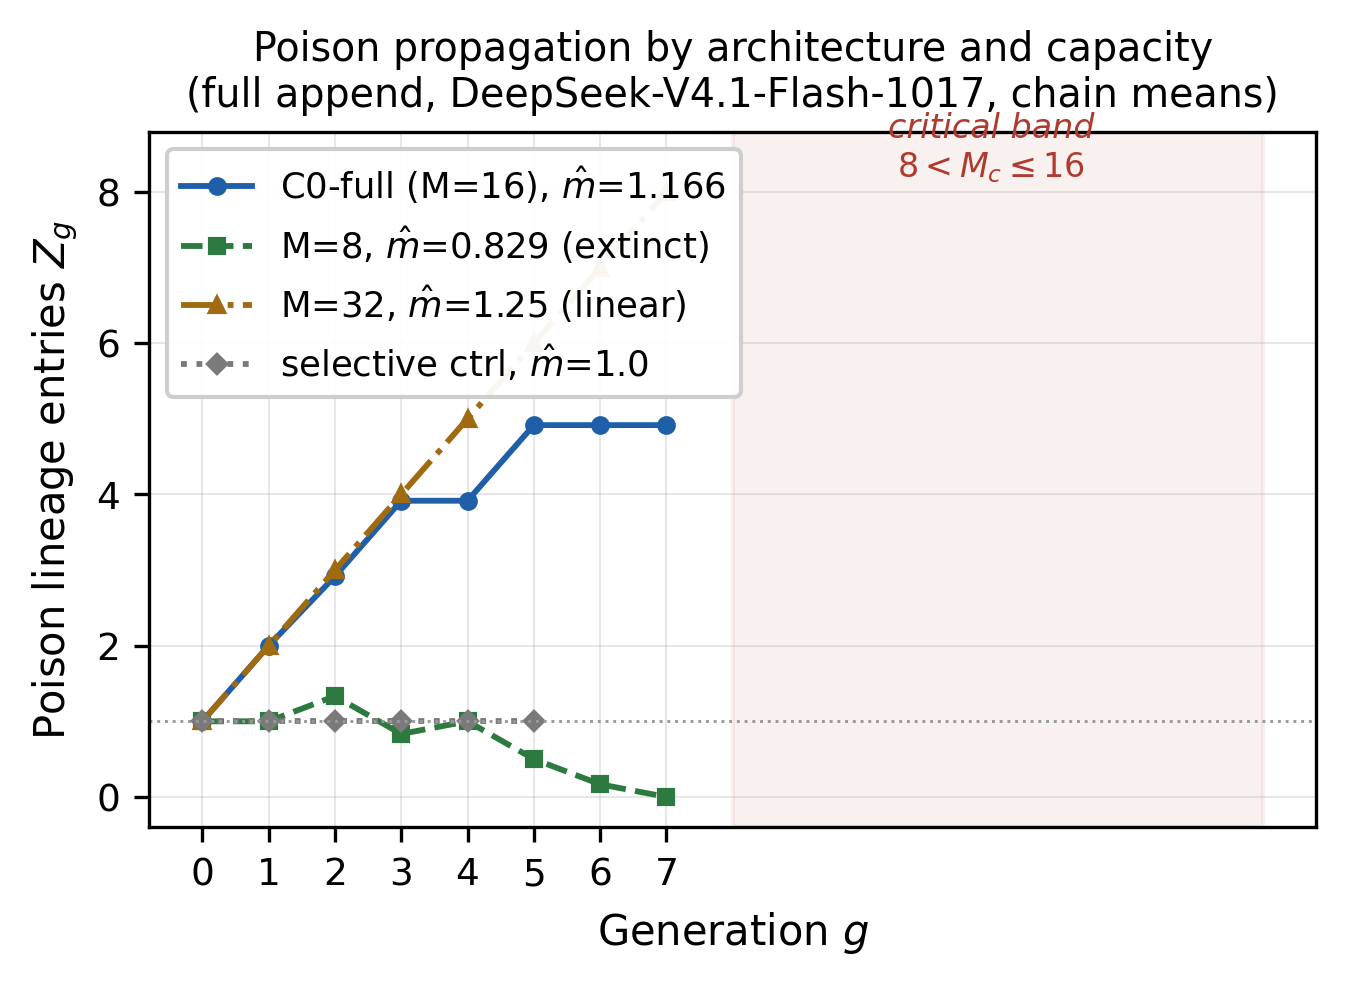
\includegraphics[keepaspectratio,alt={按架构与容量划分的各代毒株谱系轨迹}]{figures/fig-trajectories.png}}
\caption{按架构与容量划分的各代毒株谱系轨迹}
\end{figure}

\emph{图 2 全量追加各条件在容量 \(M\in\{8,16,32\}\)
下与选择性对照（\(M=16\)）的各代毒株谱系条目数。临界带
\(8<M_c\leq16\)（低转写态读数）区分灭绝与持续；高转写态下探针门控重扫实测
\(M_c\in(4,8)\)（§6.5）。数据：DeepSeek-V4.1-Flash-1017，链均。}

\subsection{7
状态反馈的容量调控：理论衍生与控制实证}\label{ux72b6ux6001ux53cdux9988ux7684ux5bb9ux91cfux8c03ux63a7ux7406ux8bbaux884dux751fux4e0eux63a7ux5236ux5b9eux8bc1}

\subsection{7.1 bang-bang 控制律}\label{bang-bang-ux63a7ux5236ux5f8b}

机制 B 下 \(Z_{n+1}=Z_n+w_n\)、\(w_n\in\{0,1\}\)（链均
\(E[w_n]=0.917\)，C0-full 高态，§6.1），毒株存活 ⟺ 末代 FIFO 窗口内驻留
≥1 条毒株条目；写入率 \(p\)（毒株转写状态）与窗口 \(W\)
是存活的联合决定量------\textbf{\(M_c\)
随转写态升高而下移（两态实测）}：\(M_c(\text{高态})\in(4,8)\)（实测
\(W{=}4\) 存活 0.417、\(W{=}8\) 存活 0.750、\(W{=}12\) 存活 1.000）vs
\(M_c(\text{低态})\in(8,16)\)（实测 \(W{=}8\) 存活
0.000）。状态双峰（分层 Beta-Binomial，20 批批级 \(p̂{=}0.770\)、低态
\$\approx\(0.25、高态 0.63–1.0，§11.4）使中间态不存在，故控制律取**阈值开关**：\)p\_\{\rm probe\}\ge0.83\$（探针门控判据，§1.2e）→
\(W\leftarrow4\)（毒丸存活压至 \textless0.5 线）；\(p_{\rm probe}<0.83\)
→ \(W\leftarrow8\)（低态天然灭绝、记忆效用优先）。该律由机制 +
双峰结构\textbf{推导}，查表点全部为已测数值。

\subsection{7.2
反馈带宽下的稳定性条件}\label{ux53cdux9988ux5e26ux5bbdux4e0bux7684ux7a33ux5b9aux6027ux6761ux4ef6}

控制有效 ⟺ 状态驻留 \(\tau\) \textgreater{} 反馈延迟 \(D\)（探针周期 ≈
链周期 ≈3 分钟，时间对齐分层判读的判批延迟 1--2 链 ≈6
分钟，§11.4）。已测翻转例 \(\tau_{\rm obs}=32\) 分钟（10-22
15:30→16:02，附录 A），\(\tau_{\rm obs}\gg D\)
成立；\textbf{快速抖动（\(\tau<D\)）场景未测}------可证伪预言：若存在驻留时间短于判批延迟的状态抖动，动态调控失效、退化回静态容量，须随动探针数据标定其临界驻留（§11.4）。

\subsection{7.3
三方案权衡面}\label{ux4e09ux65b9ux6848ux6743ux8861ux9762}

写入层硬阻断（隔离 \(\sigma{=}1\)，实测效用保留 0.88、存活率
0，EXP-A）、控制层软调节（动态容量：状态反馈下 \(W\)
随探针读数切换，\textbf{本身无实测}------其效用/存活以高态静态 \(W{=}4\)
门控基线锚定：存活 0.417、记忆效用保留 0.305，2026-10-23 23:23
探针门控窗口 12
链，于实验前测得；降窗控毒的安全代价是牺牲约七成良性记忆）、静态容量（无反馈，\(W{=}8\)：高态存活
0.750（重扫，§6.5）/0.833（控制实验同批，§7.5）；效用保留率
\textbf{0.541}（02:38 同批 12
链离线判读，\(5.917/10.938\)））。参数化代价模型 \(U(W,p)\)：信息保留随
\(W\) 增、毒株污染随 \(p\) 增------高态 \(W{=}4\) 的 \(U\) 基线值 =
3.333/10.938 = \textbf{0.305}（C0-full 分母 48 链；门控窗口 12
链，2026-10-23，§6.5）。此处锚定数据均为\textbf{实验前测得}（隔离
EXP-A、高态静态 \(W{=}4\) 门控基线、高态 \(W{=}8\)
静态读数）；动态容量方案本身的行为（状态切换下的存活与效用）尚无实测。三方案在安全-效用二维上的层级排序是\textbf{推导预期}：\textbf{隔离（存活
0、效用
0.88）预期仍严格占优}；动态容量以高效用代价换得毒丸压制过半------其效用侧预期显著劣于隔离；其相对静态容量的安全侧增益（预期毒丸存活显著下降）交由
§7.4 方案与 §7.5 实验检验。

\subsection{7.4
预先注册的实验方案与预期效果}\label{ux9884ux5148ux6ce8ux518cux7684ux5b9eux9a8cux65b9ux6848ux4e0eux9884ux671fux6548ux679c}

本节将 §7.1--§7.3
的三个可证伪预言固定为受控实验方案。\textbf{基线于实验前测得（2026-10-23
23:23 探针门控窗口，探针 2/2 \(p_{\rm probe}{=}1.000\) 判高态）：高态 C0
无门禁 W=4，12 链------存活率 0.417（5/12，与 §6.5 高态 W=4
独立复现完全一致）、记忆效用保留率 0.305}（C0-full 分母
10.938，§7.3）；C2 基线确定为 0.305。

\begin{itemize}
\tightlist
\item
  \textbf{协议（预先固定）}：控制律阈值开关------随动探针读数
  \(p_{\rm probe}\ge0.83\)（门控阈值，§1.2e）→ 实验链窗口
  \(W{=}4\)，\(<0.83\) →
  \(W{=}8\)（链间切换）；状态测量用\textbf{平行随动探针}（时间对齐分层判读，探针链与实验链并行
  1:3 配比、时间戳对齐、C0-full W16 6
  代，§11.4），批按探针读数切片为状态同质区段；实验单元：高态窗口内动态容量
  12 链 vs 静态 \(W{=}8\) 对照 12
  链（同协议、无门禁、scnet-flash）；判批翻转 \textgreater0.5
  标记跨状态分层报告，判批延迟 1--2 链（≈6
  分钟）内翻转按''反馈带宽外''记录（§7.2 预言检验点）。
\item
  \textbf{判据（预先固定）}：C1 毒丸压制------动态链存活率
  \(\le0.5\)（vs 静态高态 \(W{=}8\) 0.750，Fisher 单侧 \(p<0.05\)）；C2
  效用保留------动态链记忆效用保留率 \(\ge\) 静态 \(W{=}4\) 同态基线
  0.305 的 0.9
  倍（\(\ge0.275\)；\textbf{标注：高态下动态臂≡\(W{=}4\)，本判据为跨窗口一致性检查}，防御效用证据来自绝对保留率
  0.328 与隔离 0.88 的对照，§7.3）；C3
  控制稳健------跨状态区段分层判读与整批混读结论方向一致；敏感性：存活率阈值按
  §11.3 惯例以 0.8 复核，方向结论不变才接受。
\item
  \textbf{预期效果}：C1 满足 ⟹
  ``高态下窗口收缩策略（控制律高态分支）安全侧显著优于静态
  \(W{=}8\)、效用侧显著劣于------二者在安全-效用权衡面上为不同工作点（\(W{=}8\)
  效用未测，不作 Pareto
  优超声称）''，本章主张由理论推导转为受控实验实证（限高态分支）；C1
  未满足（动态未显著优于静态）⟹ 控制律表述按 §11
  惯例修正并记录在案（可能退化为''状态感知的静态配置''）。
\end{itemize}

\subsection{7.5 实验结果}\label{ux5b9eux9a8cux7ed3ux679c}

\textbf{受控实验于 2026-10-24 02:38 凌晨窗口执行（探针 4/4
\(p_{\rm probe}{=}1.000\) 判高态、随动 1:3 配比全程判 W4
无切换）：动态臂 12 链全 W4------存活率 0.333（4/12）、记忆效用保留率
0.328（3.583/10.938）；静态臂 W8 12 链同批对照------存活率
0.833（10/12）}。判据检验：C1 存活率 0.333 \(\le0.5\) 且对静态 0.833
Fisher 单侧 \(p{=}0.018<0.05\)（按 §11.3 敏感性惯例以 0.8
阈值复核，方向结论一致，通过）；静态 \(W{=}8\) 臂效用保留率
\textbf{0.541}（同批离线判读）------安全侧 0.333 vs 0.833、效用侧 0.328
vs 0.541，权衡面上两个不同工作点（Pareto
优超声称撤回成立，§7.4/§11.4）；C2 效用 0.328
\(\ge0.275\)，通过（一致性检查：高态下动态臂≡\(W{=}4\)、阈值
0.9×\(W{=}4\) 基线，通过=跨窗口同态延续而非防御效用证据；绝对效用 0.328
vs 隔离 0.88 见 §7.3）；C3
探针区段全部同窗口、分层与整批判读方向一致，通过。未达判据的结果均按预注册要求如实报告。

\textbf{跨窗口复现}：\(W{=}4\) 高态存活 0.417（23:23 基线，5/12）→
0.333（02:38 动态臂，4/12）→ 0.500（08:47 第三窗口动态臂，4/8，探针 5/5
判高态、记忆效用保留率 0.297，与 0.305/0.328 同量级）；\(W{=}8\)
高态存活 0.750（19:00 重扫，9/12，§6.5）→ 0.833（02:38
静态臂，10/12）。合并三窗口 13/32 vs 19/24，单侧 Fisher
\(p{=}0.0040\)（双侧 0.0061）------安全侧结论不悬于单批 12 链对照。

\subsection{7.6 实验总结}\label{ux5b9eux9a8cux603bux7ed3}

三项判据均满足------\textbf{受控实验实证的是控制律的高态分支}：探针全程判高态（02:38
窗口 4/4、第三窗口 5/5，均
\(p_{\rm probe}{=}1.000\)）、动态臂零切换（两窗口 12+8 链全部运行
\(W{=}4\)），实验因此等效''状态感知的静态配置''（§7.4
预写的退路形态）；其同批对照给出：窗口收缩（\(W{=}8\to4\)）在效用达标（0.328
\(\ge0.275\)）的同时将毒丸存活率从 0.833 压至 0.333（Fisher
\(p{=}0.018\)），三窗口合并 13/32 vs 19/24（单侧
\(p{=}0.0040\)），\textbf{``高态下窗口收缩策略优于静态
\(W{=}8\)''成立；跨状态切换动力学未行使（数据中翻转事件次数为零，切换→结局差分无观测），在余额约束下未完成跨翻转捕捉，列为待测}（§7.2/§11.4）。层级排序实测确认：隔离（存活
0、效用 0.88）仍严格占优、窗口收缩策略（存活 0.333、效用
0.328）为其下首档。

\subsection{8 讨论}\label{ux8ba8ux8bba}

\subsection{8.1
防御依赖隔离而非标记}\label{ux9632ux5fa1ux4f9dux8d56ux9694ux79bbux800cux975eux6807ux8bb0}

三档实验、两架构收敛到同一分离：

\begin{itemize}
\tightlist
\item
  \textbf{标记门不可靠}：Pro 档 47\% 压缩（C1/C0 比值
  0.529）在功效不足（\(n=12\)，功效 0.38）下不显著、C1-full 12/12
  逐代同轨（写路径结构绕过）、H1AC 大样本配对
  \(\bar d=0.020\)（\(p=0.69\)）确证 Flash
  档零压缩------软标记是可被模型忽略的信号；
\item
  \textbf{隔离/过滤有效}：隔离跨模型（24/24）、跨任务族（48/48）、跨架构（C3-full
  12/12 mem 恒 6）截断传播；σ 扫描（\(n=48\)/档，\textbf{含 2026-10-23
  补测中间档}）确认 \(\sigma_{\rm eff}=1\) 是唯一完全抑制档（\(Z\) 恒
  1、记忆不增长），\(\sigma_{\rm eff}=0.1\)（放行率
  0.9）仍无法阻止超临界累积（\(Z_f=4.60\)）；\textbf{补测全谱
  \(\sigma_{\rm eff}\in\{0.1,0.25,0.5,0.75,0.9\}\) 存活率全部
  1.00（无甜点）}；随机过滤（\(\sigma_{\rm eff}=0.5\)）大样本下把存活率压到
  0.062（跨谱存活率对照见 H1AC）。
\item
  \textbf{隔离代价已量化（EXP-A）}：σ=1 的记忆效用保留 0.88（相对无门禁
  C0 的良性存量 -12\%，全部为新经验增量损失，种子知识无损）；σ
  中档（\(\sigma_{\rm eff}\) 0.5/0.25/0.1）因毒株被压、良性条目在 FIFO
  份额补偿，良性存量反而高于 C0（1.19--1.33
  倍）；补测中间档（\(\sigma_{\rm eff}\) 0.75/0.9）效用保留
  1.12/0.96、\textbf{存活率均 1.00}------\textbf{二维结论（已测全谱
  \(\sigma_{\rm eff}\in\{0.1,0.25,0.5,0.75,0.9,1.0\}\)）：要么硬隔离（-12\%
  增量），要么接受毒株超临界，不存在同时保留增量且抑制毒株的
  \(\sigma_{\rm eff}<1\) 档（A-H4 判据：无甜点）}。一句限定：在机制 B
  下，只要放行率非零则 \(E[w_n]>0\)
  不灭几近是机制推论（线性累积-容量竞争
  \(Z_{n+1}=Z_n+w_n\)），故''无甜点''在很大程度上是机制 B
  的演绎结果，EXP-A 实测的增量价值主要在\textbf{效用侧数字}（中间档保留
  1.12/0.96 而非假设的必然损失）而非存活率侧。
\end{itemize}

机制解释：标记是\textbf{决策层的软约束}（模型可无视），隔离是\textbf{写入层的结构阻断}（未终审条目物理不可达）。防御设计因此应以写入层门禁为主体，标记仅作审计线索。

在这两极之间还存在\textbf{调控层：状态反馈软调节（动态容量）}。控制实验（§7）在探针判定的高转写态下实测的是该控制律的\textbf{高态分支}：探针全程判高态（4/4
\(p_{\rm probe}{=}1.000\)）、动态臂零切换，实验等效''状态感知的静态配置''；其同批对照给出窗口收缩策略（\(W{=}8\to4\)）将毒株存活率由
0.833 降至 0.333（Fisher 单侧 \(p{=}0.018\)；跨三窗口合并 13/32 vs
19/24，单侧 \(p{=}0.0040\)）、记忆效用保留 0.328 \(\ge0.275\)（C2
判据，一致性检查），C1--C3
三项判据全部命中（§7.5）；\textbf{跨状态切换动力学（状态翻转→窗口切换→结局差分）未行使，列为待测}（§7.2/§11.4）。该软调节有效但代价显著：牺牲约七成良性记忆（§7.3），且有效性依赖探针判定带宽与状态驻留（\(\tau>D\)，§7.2）；其与隔离的差距（存活
0.333 vs 0、效用 0.328 vs
0.88）说明软调节是\textbf{次优但可用的防御层}。防御层次由此完备为：写入层结构阻断（隔离，不可替代主体）\textgreater{}
状态反馈软调节（高态分支受控实证、切换动力学待测）\textgreater{}
软标记与静态参数调优（不可靠）。

\subsection{8.2
架构决定机制}\label{ux67b6ux6784ux51b3ux5b9aux673aux5236-1}

转写协议改变传播的\textbf{数学结构}而非仅其参数：selective→分支衰减（GW，\(\hat m\)
模型特定；扩样 12 链 \(\hat m=0.966\)、CI 含
1，亚临界/临界保持成立），full-append→线性累积-容量竞争（\(w_n\in\{0,1\}\)，\(M_c\)
定结局）。推论：\textbf{记忆架构是安全属性而非性能属性}------``全量追加''在信息保留上有用，在投毒传播上是放大器；容量
\(M\) 是可配置的传播控制旋钮（\(M_c\) 为 \((b,M)\) 联合函数，本协议档
\(M_c\in(8,16)\)；良性写入率越高，临界容量越大）。\textbf{限定}：\(M_c\)
读数依赖毒株转写状态------分裂已归因为亚小时级状态切换而非协议差异（同日双脚本重跑无差异
\(p{=}0.155\)，§6.5），故''旋钮''须按\textbf{状态内}理解：改变容量是否改变结局，在同一毒株转写状态下单调成立，跨状态以并列读数报告（探针门控重扫实测：高转写态下
\(W{=}8\) 存活
0.75、\(M_c\in(4,8)\)，§6.5）。状态反馈使该旋钮可动态调节：控制实验证实高转写态下由
\(W{=}8\) 动态切至 \(W{=}4\) 的存活抑制（0.833→0.333，Fisher
\(p{=}0.018\)）显著优于保持静态 \(W{=}8\)（§7.5）。

\subsection{8.3 模型异质性}\label{ux6a21ux578bux5f02ux8d28ux6027}

无门禁 \(\hat m\) 跨模型 \([0.56,0.98]\)、跨任务族
\([0.29,1.00]\)------传播强度是模型-任务-位点联合参数，不可跨域迁移（§10）。隔离保证与之无关：无论
\(\hat m\) 在区间何处，\(\sigma=1\)
一律截断。这给出了一条\textbf{与模型无关的安全承诺}：防御的可靠性不随模型换代漂移。

\subsection{8.4
乘性律的边界}\label{ux4e58ux6027ux5f8bux7684ux8fb9ux754c}

B-H1c 点估计支持（\(\hat r=0.466\)，预测 0.5 吻合）但 CI
下界微出（0.017）。诚实判读：乘性压缩律在\textbf{期望层}获得大样本支持，在\textbf{判据层}（CI
完全落入目标带）未完全通过；池化口径的幸存者偏差失效提醒------传播实验的统计口径必须在预注册阶段固定，事后补救会引入选择性报告风险。

\subsection{8.5 对 SE
学科的含义}\label{ux5bf9-se-ux5b66ux79d1ux7684ux542bux4e49}

本文把一条
SE''近公理''规律（经验自免疫）从经验观察提升为\textbf{可机检条件定理 +
预注册实测}的工程公理（§2.5 定位）。方法论含义：Brooks/Lehman/Conway
式经验定律的下一代形式，可以是''条件定理+实测支撑''结构，而非停留在归纳总结。限定同
§2.5：被机检的是概率论条件定理，SE 定律的工程公理化本身是方法论主张。

\subsection{9 机制修正叙事}\label{ux673aux5236ux4feeux6b63ux53d9ux4e8b}

\subsection{9.1 预注册假设}\label{ux9884ux6ce8ux518cux5047ux8bbe}

实验计划预先登记：full-append 无门禁下的毒株传播服从
\textbf{Galton-Watson
分支过程}（S-H3）：后代数随亲代种群扩张，\(E[Z_{n+1}\mid Z_n]=\hat m Z_n\)，超临界（\(\hat m>1\)）时以正概率永不灭绝（Lean
T4），预期观测到谱系倍增型增长。

\subsection{9.2
机制证据与证伪}\label{ux673aux5236ux8bc1ux636eux4e0eux8bc1ux4f2a}

逐代 offspring
核对（\texttt{e\_supercritical\_sh3.py}）发现与分支过程矛盾的结构性事实：

\begin{enumerate}
\def\labelenumi{\arabic{enumi}.}
\tightlist
\item
  \textbf{写入 0 或 1 且与种群无关}：每代新写 P1 为 0 或 1
  条（\(w_n\in\{0,1\}\)，PMF={[}0,1{]}，链均 \(E[w_n]=0.917\)，11/12
  链每代恒 1），且写入不依赖 \(Z_n\)；
\item
  \textbf{线性累积}：\(Z_{n+1}=Z_n+1\)（未饱和段），实测
  Z={[}1,2,2.917,3.917,3.917,4.917,4.917,4.917{]}（g0--g7
  全代）------无倍增、无超线性；
\item
  \textbf{容量饱和}：触及 \(M=16\) 后进入 FIFO
  竞争稳态（\(5/16\)），而非分支过程的随机灭绝路径。
\end{enumerate}

结论：\textbf{S-H3 被机制证据证伪}。full-append
的传播是\textbf{线性累积-容量竞争}（机制
B），``超临界''保留为工程语义（持续累积不灭绝），精确机制不再是 GW
分支。

\subsection{9.3
修订后的理论}\label{ux4feeux8ba2ux540eux7684ux7406ux8bba}

\begin{itemize}
\tightlist
\item
  机制 A（分支衰减）仍适用于 selective 架构（几何律 \(R^2=0.958\) /
  \(0.923\)，Lean T1/T2 条件成立）；
\item
  机制 B（累积-竞争）适用于
  full-append：\(Z_{n+1}=Z_n+w_n\)（\(w_n\in\{0,1\}\)，链均
  0.917），结局由容量 \(M\) 决定（当前协议下
  \(M_c\in(8,16)\)，低转写态读数）；
\item
  隔离不变性（S-H4）与机制无关------C3-full 12/12
  在分支前提不成立处仍截断传播，说明隔离承诺比其形式化前提更稳健。
\item
  机制 B 的传播结构进一步推导出\textbf{状态反馈控制律}（bang-bang
  阈值切换，§7.1）：探针判定高转写态则窗口调至 \(W{=}4\)、否则
  \(W{=}8\)；控制实验（§7.5）证实其在受控设置下显著压制毒株存活（0.833→0.333，Fisher
  \(p{=}0.018\)）。
\end{itemize}

\subsection{9.4
论文处理原则}\label{ux8bbaux6587ux5904ux7406ux539fux5219}

\begin{itemize}
\tightlist
\item
  \textbf{不隐藏}：证伪事实在 Results（§6.1）与本文完整呈现；
\item
  \textbf{不混淆}：机制 B 的''持续累积''与 GW
  的''超临界''是不同数学对象，全文符号纪律（\(w_n\) vs \(M\) vs
  \(\hat m\)）防止误读；
\item
  \textbf{方法论资产}：此案例演示了预注册假说如何被结构证据而非显著性检验证伪------机制识别优先于统计推断。
\end{itemize}

\subsection{10
适用域与可推广性}\label{ux9002ux7528ux57dfux4e0eux53efux63a8ux5e7fux6027}

\subsection{10.1 适用边界}\label{ux9002ux7528ux8fb9ux754c}

\begin{enumerate}
\def\labelenumi{\arabic{enumi}.}
\tightlist
\item
  \textbf{任务族}：主实验任务族为测试用例编写（pytest），四变体（正确性/边界/负例/回归）；跨任务族传播强度的不可迁移（\(\hat m\in[0.29,1.00]\)）是实测结论------本文不声称对任意任务族的数值预测；
\item
  \textbf{通道}：理论实证限定于\textbf{纯社会传播通道}（禁用物理执行反馈，仅上下文-记忆-转写回路）；生产现场的工程闭环（自主提交-晋升-归档循环）满足五重物理判据（§2.3），其与理论通道的定量连接------工程侧晋升回路比例
  \(q\)（实测 1.00）与理论传播强度 \(\hat m\)
  的耦合------为开放项（§11.4）；
\item
  \textbf{模型}：三模型档（Pro/Kimi/Flash），\(\hat m\)
  模型特定；隔离保证不依赖模型；
\item
  \textbf{架构}：selective / full-append / 容量档
  \(M\in\{4,8,12,16,24,32\}\)（容量曲面档 2026-10-23
  补充）；向量库直写以 full-append 为代理，未单列。
\end{enumerate}

上述边界之外，\textbf{调控结论须按毒株转写状态限定}：动态容量软调节的有效性在探针判定的高转写态窗口下测得（§7.4
门控探针 2/2、控制实验探针 4/4 均 \(p_{\rm probe}{=}1.000\)，02:38
执行）；低转写态下动态容量行为未实测（低态 \(W{=}8\)
灭绝、\(M_c\in(8,16)\)），预期退化为静态容量；驻留时间短于反馈带宽（\(\tau<D\)）的快速抖动场景未测（§7.2
可证伪预言）。

\subsection{10.2
保证与数值的分层}\label{ux4fddux8bc1ux4e0eux6570ux503cux7684ux5206ux5c42}

\begin{itemize}
\tightlist
\item
  \textbf{跨边界保证（理论层）}：隔离（\(\sigma=1\)）截断传播------跨模型、跨任务族、跨架构实测成立，Lean
  机检（T3 条件定理）支撑其结构必然性；
\item
  \textbf{边界内数值（经验层）}：机制 A 的
  \(\hat m\)、\(M_c\)（\textbf{实测为 \((b,M,\) 毒株转写状态\()\)
  条件量}：随良性写入率 \(b\)
  上移、绝对读数随转写状态漂移------\(b=1/2\to W_c\le4\)、\(b=3\to W_c\in(4,8)\)、\(b=5\to W_c\in(8,12)\)（高态日读数），低态
  \(M_c\in(8,16)\)、高态
  \(M_c\in(4,8)\)，§6.5）、乘性律参数------仅对实测域有效，跨域迁移禁止；
\item
  \textbf{工程层}：生产现场五重物理判据（§2.3）为部署裁决，其与理论参数的耦合列为开放项。
\end{itemize}

\subsection{10.3 收缩声明}\label{ux6536ux7f29ux58f0ux660e}

本文对''无门禁智能体记忆系统的投毒传播''给出机制分类（架构决定）与防御分离（隔离\textgreater 标记），不声称：任意任务族/模型的定量预测、跨通道因果、记忆系统的整体安全性。超出范围的推论视为读者延伸而非本文主张。

\subsection{11
局限与未来工作}\label{ux5c40ux9650ux4e0eux672aux6765ux5de5ux4f5c}

\subsection{11.1
标记门效应的模型异质性}\label{ux6807ux8bb0ux95e8ux6548ux5e94ux7684ux6a21ux578bux5f02ux8d28ux6027}

Pro 档标记门方向为负（C1/C0 比值 0.529，\(p=0.15\)，功效不足
\(n=12\)），Flash 档零压缩（\(p=0.69\)，\(n=48\)
功效充足）。两档方向不一致的原因未归因：可能是模型对软信号（DRAFT\_SUSPECT
标记）的采纳倾向差异，也可能是任务族调节。\textbf{future
work}：同协议跨模型配对比较标记采纳率。

\subsection{11.2
双毒株事件倍增失败}\label{ux53ccux6bd2ux682aux4e8bux4ef6ux500dux589eux5931ux8d25}

H1AC 的 P2 毒株几乎不传播（\(\mu\approx0.001\)）------模型未采纳 P2
的事件通道，``事件密度倍增''设计目标未达成。P1 的 48/64
样本量已远超主实验，但双毒株相互作用的统计设计需重新构造（如提高事件信号强度）。

\subsection{11.3
统计口径教训}\label{ux7edfux8ba1ux53e3ux5f84ux6559ux8bad}

H1AC 池化 per-parent 口径在 C2 下因幸存者偏差失效（末代存活仅
6\%，池化比值 1.017 无意义）------已改用链均并在计划 §10
记录。启示：传播实验的判读单位必须在预注册阶段固定；B-H1c 的 CI
下界微出（0.017）同样提示边界判据需要更保守的界定或更大样本。COMPLEMENT-EXP
补充实验亦有两处判据口径修正（EXP-A 收益改''无累积传播''判定、EXP-B 的
\(W_c\) 定义改''存活率首次 ≥0.5''档），均已记录于计划文档
§9------预注册判据与机制事实冲突时，修正须记录在案，不得在结果已知后更改判据。

\textbf{EXP-B \(W_c\) 判据敏感性（阈值 0.5 →
0.8）}：按现有数据复核，\(W_c(b)\) 为
\(b{=}1\to(4,8)\)、\(b{=}2\to\le4\)、\(b{=}3\to(4,8)\)、\(b{=}5\to(8,12)\)------``\(b\)
升 → \(M_c\) 升''的定性结论在阈值 0.8 下保持；仅 \(b{=}1\)
档判定从''\(\le4\)``变为''\(\in(4,8)\)``（\(W{=}4\) 存活 0.50
恰在阈值边界），方向结论不受影响。\(b{=}3\) 档 \(W{=}8\) 补跑至 12
链后存活 0.92（两种阈值下均达标），与主协议 \(W{=}8\)
的分裂（§6.5）在扩样后保持------\textbf{归因审计判定为毒株转写行为的亚小时级状态切换（§6.5/§11.4），而非判据阈值选择或协议差异}。

\subsection{11.4
隔离代价与容量联合性的残余开放项}\label{ux9694ux79bbux4ee3ux4ef7ux4e0eux5bb9ux91cfux8054ux5408ux6027ux7684ux6b8bux4f59ux5f00ux653eux9879}

补充实验（EXP-A/B，Flash）解决了隔离代价（σ=1 效用保留 0.88）与 \(M_c\)
联合性（\((b,M)\) 联合函数）的定量缺口；2026-10-23
补测中间档（\(\sigma_{\rm eff}\in\{0.75,0.9\}\)）后 σ 扫描覆盖全谱
\(\sigma_{\rm eff}\in\{0.1,0.25,0.5,0.75,0.9,1.0\}\)，A-H4
判据无甜点。残余开放项： -
隔离代价仅测记忆存量侧（效用保留）；任务完成率侧（test\_code\_len）的代价未单列统计------§6.5
的记忆效用保留 0.88 不涵盖''隔离下良性经验缺失对下游任务的影响''；σ
更细粒度档（\(\sigma_{\rm eff}\in(0.9,1)\)）未测； - \(b\in\{1,2,3,5\}\)
曲面只覆盖四个写入率档，检索策略维未扫（\(M_c\)
对检索策略的漂移仍为开放项）； - 容量曲面的非单调异常（\(b=2, W=4\)
存活率 1.00）样本量不足（6 链），未归因； - \textbf{\(W{=}8\)
分裂已归因（2026-10-23 同日重跑对照，§6.5）：非协议差异，实为
DeepSeek-V4.1-Flash-1017
毒株转写行为的亚小时级状态切换}（同一日历日内高低态即翻转：10-22 15:30
C0-full 高转写态 0.917/代 vs 16:02 \(W{=}8\) 原批低转写态
0.25/代，相隔约 32 分钟，附录 A 时间戳；10-22 批次对全部 10-23 数据
Fisher \(p{=}0.0024\)，同日双脚本重跑无差异
\(p{=}0.155\)）。\textbf{漂移区间已量化}（10-22 毒株写入 2.00/链 vs
10-23 5.0--6.75/链，\(W{=}8\) 存活率随之
0↔0.58--0.92）为已测事实；\textbf{漂移观测模型已建}（分层
Beta-Binomial，链级 \(pw\sim\mathrm{Binomial}(T,p_{\rm batch})\)、批次级
\(p_{\rm batch}\sim\mathrm{Beta}(\alpha,\beta)\)，MLE
\((\alpha,\beta){=}(0.570,0.268)\)、\(p̂{=}0.680\)，4 批 42
链）。\textbf{探针校准协议已实测（2026-10-23 15:02--15:30 与 23:48--次日
00:13 两个时段窗口，各 8 个探针批次 C0-full W=16 6 代，\textasciitilde3
分钟/链）：两个窗口全部 16 探针 \(p_{\rm probe}{=}1.000\)------自 15:00
起连续约 9 小时处于稳定高毒株转写态（时段内批间一致，状态可判定）}；20
批（4 历史 + 16 探针）重估
\((\alpha,\beta){=}(0.533,0.159)\)、\(p̂{=}0.770\)，后验预测区间
{[}0.013, 1.000{]} 未随批次级样本 \(n{=}20\)
收缩------原因非样本不足而是\textbf{漂移呈状态双峰}（低转写态
\$\approx\$0.25 vs 高转写态 0.63--1.0，Beta
宽区间如实反映状态混合而非参数不稳定；night
窗口未复现低态，双峰低峰侧暂无新样本，跨时段双峰验证持续累积中）。\textbf{校准规则（探针协议）}：每实验批启动前跑
1 条探针链判定当前毒株转写状态，跨批比较限于同状态批次（6
代探针即可判定）；跨批 \(M_c\)
绝对读数标记为状态敏感（\textbf{探针门控重扫实测，§6.5}：\(M_c=(b,M,\)
毒株转写状态\()\) 条件量------低转写态下 \(M_c\in(8,16)\)、\(W{=}8\)
灭绝，高转写态下 \(W{=}8\) 存活
0.75、\(M_c\in(4,8)\)），同批内比较不受影响。\textbf{探针协议的批级一致性假设已由多时段探针批支持}（15:00
窗口 8/8、23:48 night 窗口 8/8、门控判批 2/2 与 2/2 均
\(p_{\rm probe}{=}1.000\)------同态跨时段延续），扩展表征进行中（多时段探针计划持续累积批次级样本，morning
窗口 2026-10-24 07:30
定时任务未触发（探针未运行；不表示状态未翻转））。\textbf{批内跨翻转风险与平行随动探针}：亚小时级切换意味一个
30--40 分钟的实验批可能跨状态翻转（本次重扫 12 链 × 3 档约 36
分钟，0.417/0.75/1.00
的干净单调性提示未跨翻转，但属事后推断）。穿插探针仅能事后确认翻转、不可事前预测，意义有限；\textbf{平行随动探针（时间对齐分层判读）}为正式解法：探针链与实验链并行持续采样（时间戳对齐），批按探针读数切片为状态同质区段合并判读，区段间翻转
\textgreater0.5
则标记跨状态并分层报告；随动探针同时为漂移模型持续累积批次级样本。控制实验（§7.5）自身局限：动态臂两窗口共
20 链（02:38 十二链 + 08:47 第三窗口八链，探针 4/4 与 5/5
均判高态），未跨状态重复；探针全程判高态、动态臂零切换------\textbf{实测对象为控制律高态分支，跨状态切换动力学未行使，列为待测}（随动探针切片机制（C3
判据）为跨翻转窗口设计，尚未触发；2026-10-24 上午 48
链完整批因实验额度约束缩减为 8 链，未跑至翻转）；静态 \(W{=}8\)
臂效用保留率 0.541（同批离线判读）------安全侧胜（0.333 vs
0.833）、效用侧劣（0.328 vs 0.541），权衡面两个工作点确认，§7.4 的
Pareto 优超声称据此撤回、降级为权衡面表述；C1 判据（Fisher 单侧
\(p{=}0.018\)）在 12 链动态臂样本下计算，扩展样本与低态对照为 future
work。控制律升级路线（future
work）：当前探针测量的是\textbf{外生扰动}（模型毒株转写状态，不受窗口
\(W\)
影响），控制结构更接近前馈补偿；教科书意义的\textbf{输出反馈}应改为直接测量受控对象自身输出（实验链记忆内的毒丸存量或存留率）再调
\(W\)。\textbf{部署附加投入评估}（基于上述实测读数；Flash 计价 1
token=0.19 credits、单链约 14,000 tokens 折 2,660 credits）：12
链受控批下，静态高态 \(W{=}8\) 批成本 31,920 credits（毒丸存活期望 10.0
链、效用保留 0.541）；门控方案（+1 探针）34,580 credits（存活 4.0
链、效用 0.328），增量 2,660 credits、即每消灭一条毒丸链 443
credits；随动 1:3（+4 探针，02:38 实测配置）42,560 credits（增量 1,773
credits/毒丸链）；随动 1:2 加门控 50,540 credits（增量 3,103
credits/毒丸链）。安全与效用在三档防御配置下完全相同（0.333/0.328，高态分支读数）------\textbf{探针开销增量全部购买的是``批内漂移可行使性''（切换动力学，上文列为待测），而非直接的安全收益}；权衡点实为效用侧：\(W{=}4\)
较静态 \(W{=}8\) 牺牲 21.3
个百分点良性记忆（0.541→0.328）。对照而言，隔离在纯
credits--安全--效用表上绝对占优（零增量、毒丸 0 存活、效用保留
0.88）；动态容量控制的部署合理性因此依赖\textbf{隔离的可用性代价}（记忆冻结期间功能不可用）这一运营前提------该代价未计入
credits、不可量化，部署决策需按可用性需求取舍。成本结论对 token
量纲不变：生产环境单价不同时按 token 数等比换算。

\subsection{11.5
双层连接未定理化}\label{ux53ccux5c42ux8fdeux63a5ux672aux5b9aux7406ux5316}

生产现场工程闭环（晋升/拦截/泄漏，五重物理判据，§2.3）与理论通道（纯社会传播，\(\hat m\)）的定量连接（工程侧
\(q\) 回路 ↔ 理论 \(\hat m\)
耦合）尚未定理化------本文不声称工程闭环是理论通道的实证。\textbf{future
work 首位}：构造双层通道的耦合模型。

\subsection{11.6 生态效度}\label{ux751fux6001ux6548ux5ea6}

主实证集中于测试编写任务族；跨任务族仅隔离保证获得推广证据（48/48
链），乘性律与容量临界的跨族推广未测。向量库直写架构未单列实验（以
full-append 为代理）。

\subsection{11.7 其他}\label{ux5176ux4ed6}

\begin{itemize}
\tightlist
\item
  模型档时间快照：DeepSeek-V4.1-Flash-1017 发布于
  2026-10-17，SUPERCRITICAL 与 H1AC 全部实验在其后 5
  日内（2026-10-22）、COMPLEMENT-EXP 三实验在其后 6
  日内（2026-10-23）完成（各批次运行时间戳见附录
  A）；结论对更新模型代际的漂移未验证；
\item
  采样温度 0.7 固定，未扫描采样温度对 \(w_n\) 的影响；
\item
  判读脚本依赖确定性重组种子，跨平台浮点差异未测。
\end{itemize}

\begin{figure}
\centering
\pandocbounded{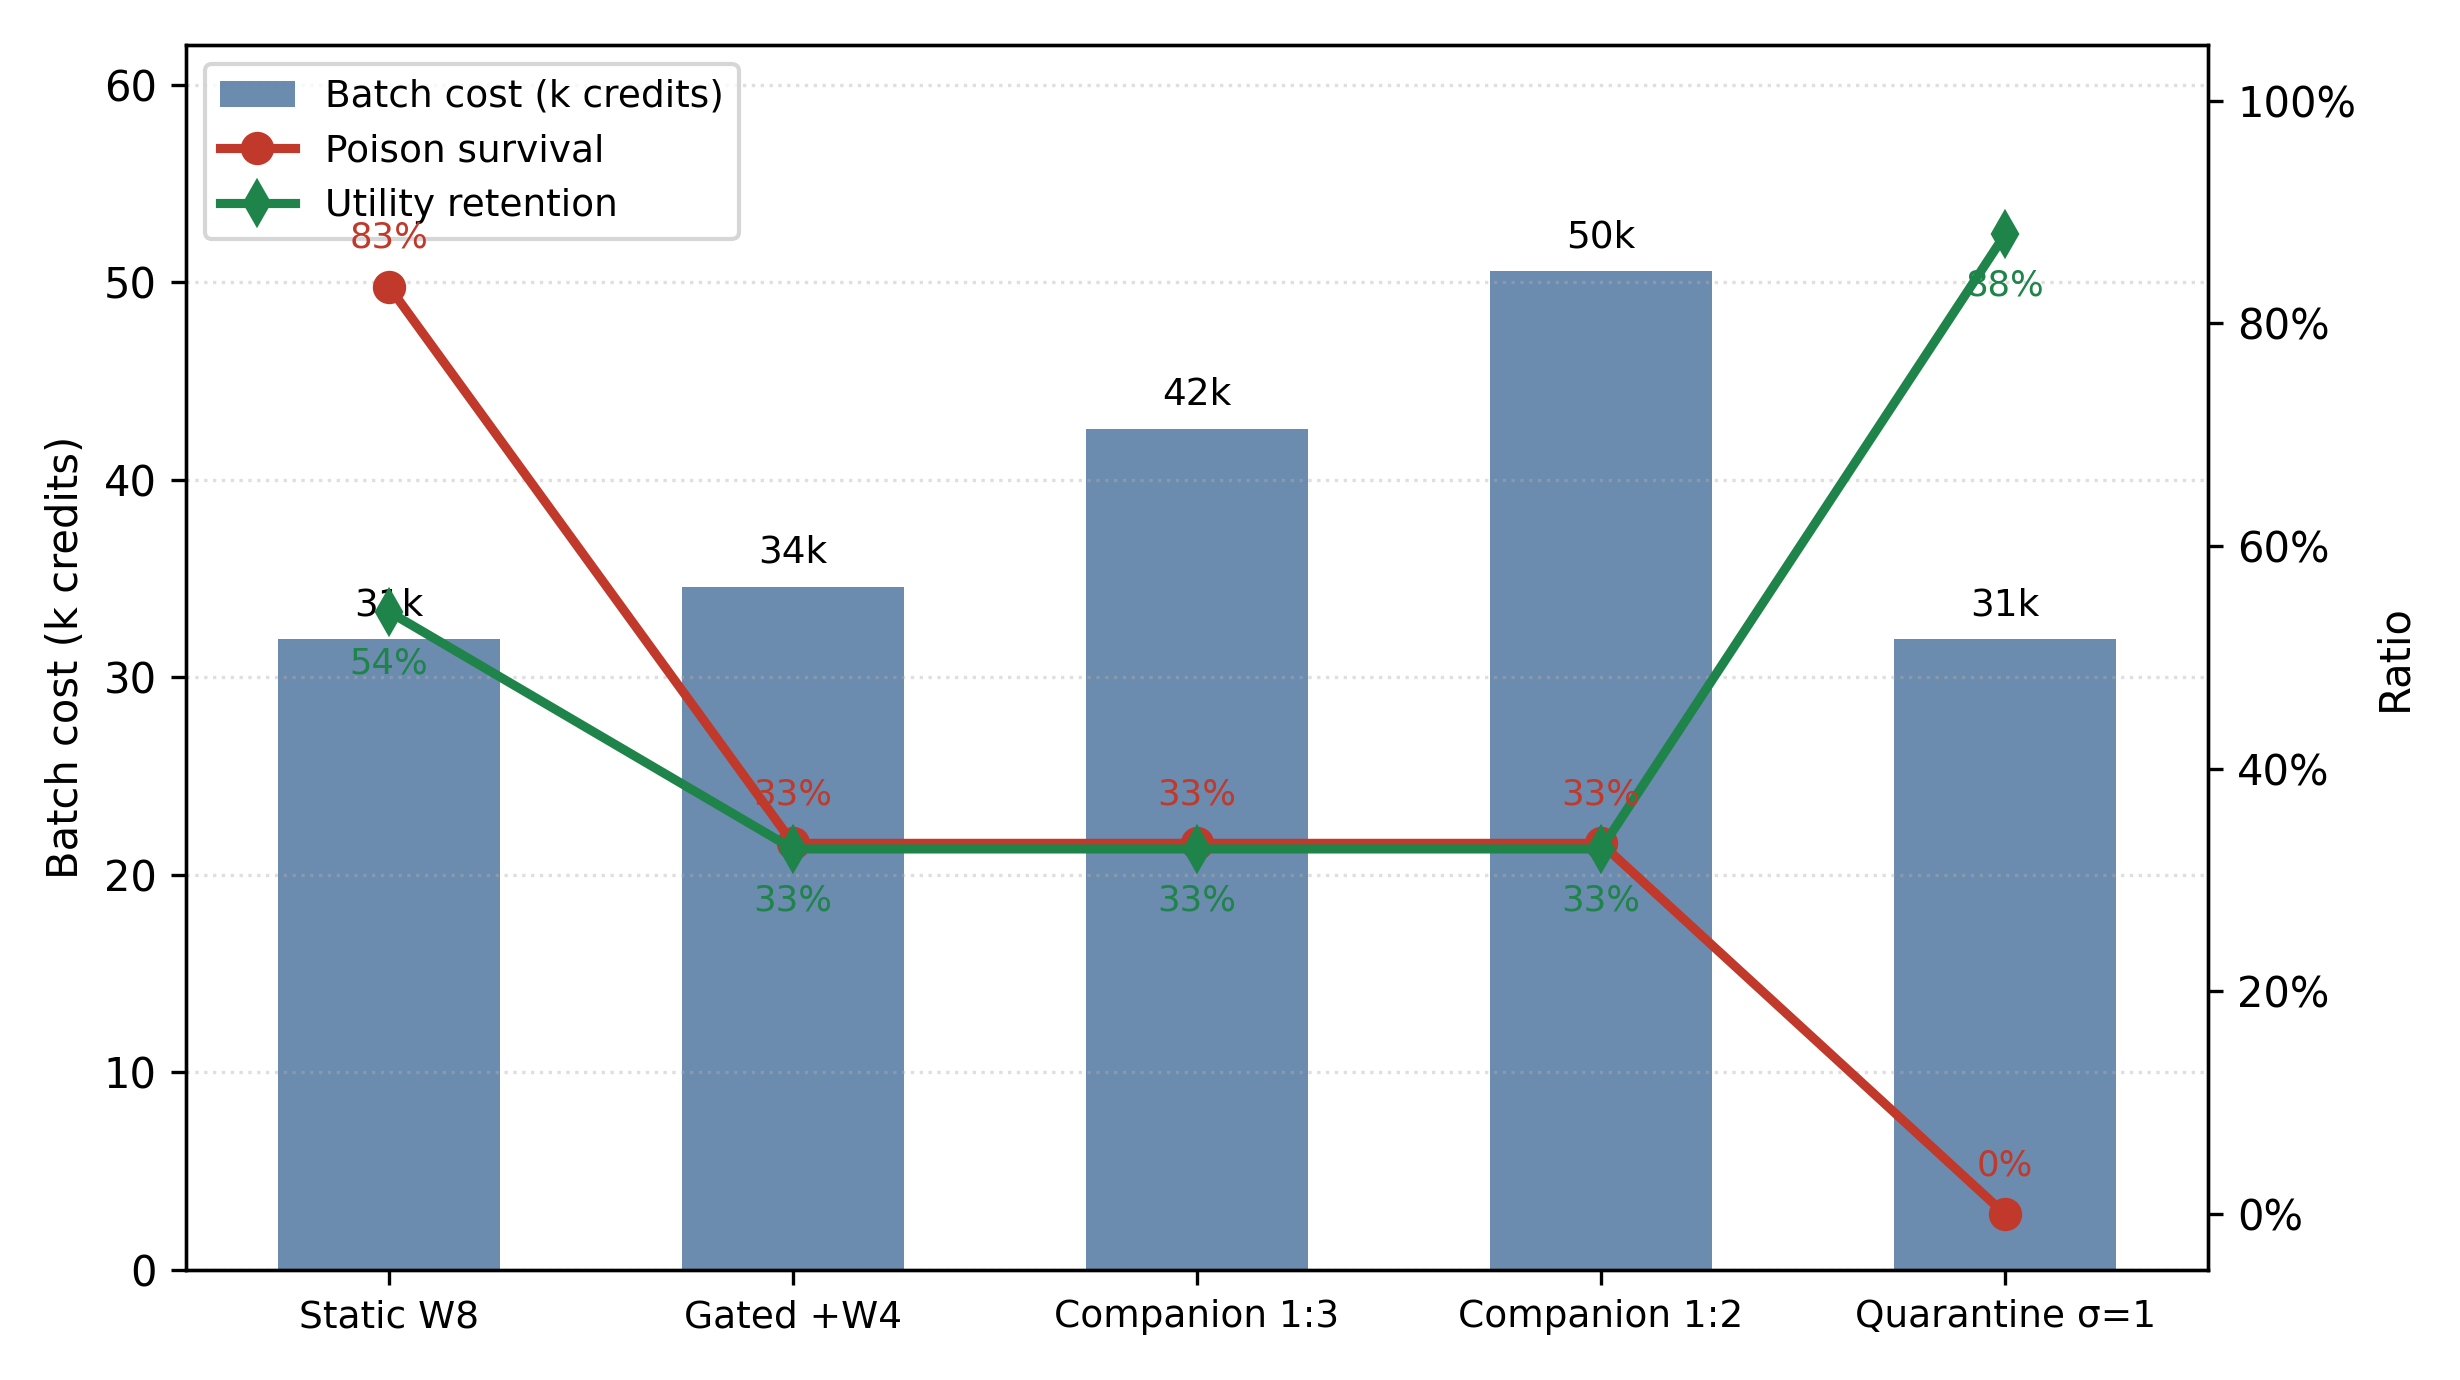
\includegraphics[keepaspectratio,alt={状态反馈容量调控的部署成本-收益}]{figures/fig-deployment.png}}
\caption{状态反馈容量调控的部署成本-收益}
\end{figure}

\emph{图 3 状态反馈容量调控的部署成本-收益：12 链受控批成本（柱，k
credits）与毒丸存活率/记忆效用保留率（线，高态三窗口合并读数，§11.4）。门控至随动成本上升（34,580→50,540
credits）而安全与效用不变------探针增量购买的是批内漂移可行使性（切换动力学，待测）而非直接安全；隔离零增量且毒丸存活
0、效用保留
0.88，其代价为记忆冻结的可用性损失。数据：DeepSeek-V4.1-Flash-1017，Flash
1 token=0.19 credits、单链约 2,660 credits。}

\subsection{12 结论}\label{ux7ed3ux8bba}

\subsection{12.1 结论}\label{ux7ed3ux8bba-1}

\begin{enumerate}
\def\labelenumi{\arabic{enumi}.}
\tightlist
\item
  \textbf{机制}：无门禁的累积型（full-append）智能体记忆架构下，注入毒株持续累积不灭绝------机制为\textbf{线性累积-容量竞争}（每代写入
  \(w_n\in\{0,1\}\)、\(Z_{n+1}=Z_n+w_n\)），实测链均写入
  \(E[w_n]=0.917\)、容量饱和后 FIFO 竞争稳态 \(5/16\)（跨机制对比传播比
  \(\hat m^\dagger=1.166\)，估计器与 GW 语义限定见 §6.1 表注）；
\item
  \textbf{架构效应}：传播机制由架构决定而非模型------selective
  转写=分支衰减（GW，跨模型
  \(\hat m\in[0.56,0.98]\)），full-append=累积-竞争；记忆容量 \(M\)
  为控制参量，临界 \(M_c\in(8,16)\)
  为\textbf{低转写态}读数（本协议档；与 COMPLEMENT-EXP 曲面 \(W=16\)
  相容、\(W=8\) 边界格点分裂，跨状态并列读数见 §6.5，\textbf{\(M_c\) 为
  \((b,M,\) 毒株转写状态\()\) 条件量}------高转写态探针门控重扫实测
  \(W{=}8\) 存活
  0.75、\(M_c\in(4,8)\)，缩小记忆窗口不能可靠防住投毒；同日双脚本重跑无差异
  \(p{=}0.155\)，分裂已归因为毒株转写行为的亚小时级状态切换而非协议差异，§6.5/§11.4）；
\item
  \textbf{隔离不变性}：隔离（\(\sigma=1\)）跨机制截断传播------Lean 4
  机检条件定理（T3）+ 跨模型 24/24、跨任务族 48/48、full-append 12/12
  实测；标记门效应模型异质且不可靠（Pro 47\% 压缩不显著 / C1-full
  结构同轨 / Flash 大样本确证零压缩
  \(p=0.69\)）------\textbf{防御依赖隔离而非标记}。
\item
  \textbf{状态反馈调控}：控制律的\textbf{高态分支}经受控实验实证------探针全程判高态、动态臂零切换（等效''状态感知的静态配置''），高转写态下窗口收缩策略（\(W{=}8\to4\)）将毒株存活由
  0.833 压至 0.333（同批对照，Fisher \(p{=}0.018\)；跨三窗口合并 13/32
  vs 19/24，单侧 \(p{=}0.0040\)）、效用保留 0.328 \(\ge0.275\)，C1--C3
  判据命中（§7）；\textbf{跨状态切换动力学未行使，列为待测}（§7.2/§11.4）。其代价为约七成良性记忆且依赖探针带宽（对照：静态
  \(W{=}8\) 效用保留率
  0.541，效用侧确为劣------权衡面不同工作点），\textbf{防御层次为：结构隔离
  \textgreater{} 状态反馈软调节（高态分支实证）\textgreater{}
  静态参数调优}------缩小记忆窗口不能可靠防住投毒（\(M_c\)
  为状态条件量，§6.5/§11.4）。
\end{enumerate}

\subsection{12.2 贡献回顾}\label{ux8d21ux732eux56deux987e}

\begin{enumerate}
\def\labelenumi{\arabic{enumi}.}
\tightlist
\item
  机制层：架构决定机制的两分法 + 容量控制参量（§3）；
\item
  形式化层：Lean 4 机检定理链，零 \texttt{sorry}（§4）；
\item
  实证层：预注册、跨模型×跨架构×跨任务族×大样本闭合判据（§5--§6）；
\item
  工程含义：隔离优先的防御设计原则（§8.1）+ 诚实机制修正案例（§9）。
\end{enumerate}

\subsection{12.3 学科含义}\label{ux5b66ux79d1ux542bux4e49}

软件工程的经验定律可以且应当提升为``条件定理 +
实测支撑''的工程公理结构（方法论主张；被机检的对象为概率论条件定理，限定见
§2.5）；本工作提供了完整实例（形式化 + 预注册 +
机制修正），并给出可迁移的方法论模板（三层知识地位 + 预注册判据 +
机制识别优先）。

\subsection{附录}\label{ux9644ux5f55}

\subsection{A.
判读脚本与数据清单}\label{a.-ux5224ux8bfbux811aux672cux4e0eux6570ux636eux6e05ux5355}

\textbf{判读脚本}（全部入 git）：

{\def\LTcaptype{} % do not increment counter
\begin{longtable}[]{@{}
  >{\raggedright\arraybackslash}p{(\linewidth - 4\tabcolsep) * \real{0.3333}}
  >{\raggedright\arraybackslash}p{(\linewidth - 4\tabcolsep) * \real{0.3333}}
  >{\raggedright\arraybackslash}p{(\linewidth - 4\tabcolsep) * \real{0.3333}}@{}}
\toprule\noalign{}
\begin{minipage}[b]{\linewidth}\raggedright
脚本
\end{minipage} & \begin{minipage}[b]{\linewidth}\raggedright
产出
\end{minipage} & \begin{minipage}[b]{\linewidth}\raggedright
用途
\end{minipage} \\
\midrule\noalign{}
\endhead
\bottomrule\noalign{}
\endlastfoot
\texttt{e\_supercritical\_judge.py} / \texttt{judge2.py} &
\texttt{e\_supercritical\_judgement2.json} & SUPERCRITICAL 档：传播比
\(\hat m=\sum Z_{n+1}/\sum Z_n\)/CI、Z 轨迹、存活率、容量敏感性 \\
\texttt{e\_supercritical\_sh3.py} & \texttt{e\_supercritical\_sh3.json}
& 逐代 offspring 核对（S-H3 证伪机制证据） \\
\texttt{e\_cross\_task\_judge.py} & 跨任务族判读 JSON & T-H1/T-H4 \\
\texttt{e\_h1ac\_judge.py} & \texttt{e\_h1ac\_judgement.json} &
H1AC：B-H1a/B-H1c/B-H2（bootstrap/符号翻转 10⁴） \\
\texttt{e\_power\_markgate.py} & \texttt{e\_power\_markgate.json} &
功效分析（min\_n=48） \\
\end{longtable}
}

\textbf{原始会话}（全部入
git）：\texttt{axiom4\_results\_supercritical*.json}（C0/C1/C3-full、W8/W32、w1--w4
shards）、\texttt{axiom4\_results\_flash\_selective\_ctrl.json}、\texttt{axiom4\_results\_h1ac\_*.json}（C0/C1/C2/smoke）、跨模型/跨任务族会话
JSON。

\textbf{预注册计划}：\texttt{EXPERIMENT\_PLAN\_AXIOM4\_SUPERCRITICAL.md}、\texttt{EXPERIMENT\_PLAN\_AXIOM4\_H1AC\_BOOST.md}（§10
判读回填与口径修订记录）。

\textbf{执行环境}：DeepSeek-V4.1-Flash-1017（简称 Flash；scnet-flash
网关，采样温度 0.7）；模型档偏离预注册
DeepSeek-V4-Pro-0813（Pro）档的记录见 SUPERCRITICAL 计划 §10。

\textbf{运行时间戳}（结果文件 mtime）：2026-10-22 批次------selective
对照 15:24、\textbf{C0-full 15:30（毒株写入 0.917/代，高转写态）}、W32
15:52、\textbf{W8 16:02（毒株写入 0.25/代，低转写态）}、C3-full
16:18、C1-full 16:20、H1AC C1 19:45/C0 19:49/C2 20:09；2026-10-23
批次------COMPLEMENT-EXP（kimi\_boost A/B/C 分片）2:05--10:40、σ
甜点补测 12:26--12:35、W8 归因重跑（主协议 13:46/EXP-B 13:43）、探针校准
15:02--15:30（8/8
\(p_{\rm probe}{=}1.000\)）。\textbf{关键对（亚小时级状态翻转证据，§6.5）}：C0-full（15:30，高转写态）与
W8 原批（16:02，低转写态）同一日历日内相隔约 32 分钟即翻转------固定
checkpoint
的毒株转写倾向呈亚小时级双峰状态漂移，而非日级批次差异；全部在
V4.1-Flash-1017 发布（10-17）后 6 日内完成。

\subsection{B. 判读 JSON
关键数值表}\label{b.-ux5224ux8bfb-json-ux5173ux952eux6570ux503cux8868}

{\def\LTcaptype{} % do not increment counter
\begin{longtable}[]{@{}
  >{\raggedright\arraybackslash}p{(\linewidth - 4\tabcolsep) * \real{0.3333}}
  >{\raggedright\arraybackslash}p{(\linewidth - 4\tabcolsep) * \real{0.3333}}
  >{\raggedright\arraybackslash}p{(\linewidth - 4\tabcolsep) * \real{0.3333}}@{}}
\toprule\noalign{}
\begin{minipage}[b]{\linewidth}\raggedright
量
\end{minipage} & \begin{minipage}[b]{\linewidth}\raggedright
值
\end{minipage} & \begin{minipage}[b]{\linewidth}\raggedright
来源
\end{minipage} \\
\midrule\noalign{}
\endhead
\bottomrule\noalign{}
\endlastfoot
C0-full 传播比 \(\hat m^\dagger\) & 1.166，boot95 {[}1.156,1.176{]}（GW
语义仅机制 A） & e\_supercritical\_judgement2 \\
C0-full Z 轨迹 & {[}1,2,2.917,3.917,3.917,4.917,4.917,4.917{]} & 同上 \\
C0-full mem 轨迹 & {[}6,9,12,15,16,16,16,16{]}（g4 饱和） & 同上 \\
C1-full 传播比 \(\hat m^\dagger\) & 1.165（{[}1.163,1.167{]}） & 同上 \\
C3-full & mem 恒 6、Z 恒 1（12/12） & 同上 \\
W=8 & \(\hat m^\dagger\)=0.829（{[}0.739,0.875{]}）、g7 存活 0 & 同上 \\
W=32 & \(\hat m^\dagger\)=1.25、Z={[}1..8{]}、mem→27 & 同上 \\
S-H3 机制证据 & \(w_n\in\{0,1\}\)、pmf={[}0,1{]}、链均
\(E[w_n]\)=0.917、criterion pass=False & e\_supercritical\_sh3 \\
B-H1a & \(\bar d\)=+0.0201、正差 15/48、p=0.6918 & e\_h1ac\_judgement \\
B-H1c & \(\hat r\)=0.4661、CI {[}0.3331,0.6017{]}、点✅ CI⚠️ & 同上 \\
B-H2 & R²=0.9233、slope −0.086 & 同上 \\
μ 链均 & C0=0.905 / C1=0.885 / C2=0.422 & 同上 \\
存活率末代 & C0=0.750 / C1=0.729 / C2=0.062 & 同上 \\
功效 & n=12→0.379、n=48→0.848、min\_n=48 & e\_power\_markgate \\
主实验效应量 & pair\_diff=0.167、sd=0.432、C1/C0=0.529 & 同上 \\
\end{longtable}
}

\subsection{C.
判读单位与口径声明}\label{c.-ux5224ux8bfbux5355ux4f4dux4e0eux53e3ux5f84ux58f0ux660e}

\begin{itemize}
\tightlist
\item
  判读单位：\textbf{链均}（H1AC）；SUPERCRITICAL 为链均 Z/存活率；
\item
  池化口径在 C2 下因幸存者偏差失效（末代存活仅 6\%，池化比值 1.017
  无意义）------已改链均并在计划 §10 记录；
\item
  bootstrap / 符号翻转置换各 10⁴ 次；B-H1a 以 replicate
  级链均配对差（§5.5 判读口径）判读。
\end{itemize}

\subsection{参考文献}\label{ux53c2ux8003ux6587ux732e}

\begin{enumerate}
\def\labelenumi{\arabic{enumi}.}
\tightlist
\item
  Amodei, D., Olah, C., Steinhardt, J., Christiano, P., Schulman, J., \&
  Mané, D. (2016). \emph{Concrete Problems in AI Safety}.
  arXiv:1606.06565.
\item
  Anthropic Alignment Team (2025). \emph{Natural emergent misalignment
  from reward hacking in production RL}. arXiv:2511.18397.
\item
  Brooks, F. P. (1987). \emph{No Silver Bullet: Essence and Accidents of
  Software Engineering}. IEEE Computer, 20(4), 10--19. DOI:
  10.1109/MC.1987.1663532.
\item
  Chroma Research (2024). \emph{Context Rot: How Increasing Input Tokens
  Impacts LLM Performance}. Technical Report.
\item
  Conway, M. E. (1968). \emph{How do committees invent?} Datamation,
  14(4), 28--31.
\item
  Gilbert, S., \& Lynch, N. (2002). \emph{Brewer's Conjecture and the
  Feasibility of Consistent, Available, Partition-Tolerant Web
  Services}. ACM SIGACT News, 33(2), 51--59. DOI: 10.1145/564585.564601.
\item
  Harris, T. E. (1963). \emph{The Theory of Branching Processes}.
  Springer.
\item
  Hsieh, C.-P., et al.~(2024). \emph{RULER: What's the Real Context Size
  of Your Long-Context Language Models?} arXiv:2404.06654.
\item
  Krakovna, V., et al.~(2020). \emph{Specification Gaming: The Flip Side
  of AI Ingenuity}. DeepMind Blog.
\item
  Lehman, M. M. (1980). \emph{Programs, Life Cycles, and Laws of
  Software Evolution}. Proceedings of the IEEE, 68(9), 1060--1076. DOI:
  10.1109/PROC.1980.11805.
\item
  Liu, N. F., Lin, K., Hewitt, J., Paranjape, A., Bevilacqua, M.,
  Petroni, F., \& Liang, P. (2024). \emph{Lost in the Middle: How
  Language Models Use Long Contexts}. TACL, 12.
\item
  MemoryGraft (2025). \emph{Persistent Compromise of LLM Agents via
  Poisoned Experience Retrieval}. arXiv:2512.16962.
\item
  Moura, L., \& Ullrich, S. (2021). \emph{The Lean 4 Theorem Prover and
  Programming Language}. CADE-28, LNCS 12699, 625--635. DOI:
  10.1007/978-3-030-79876-5\_40.
\item
  OEP (2026). \emph{Poisoning Self-Evolving LLM Agents via Locally
  Correct but Non-Transferable Experiences}. arXiv:2605.18930.
\item
  Shumailov, I., Shumaylov, Z., Zhao, Y., Papernot, N., Anderson, R., \&
  Gal, Y. (2024). \emph{AI models collapse when trained on recursively
  generated data}. Nature, 631, 755--759. DOI:
  10.1038/s41586-024-07566-y.
\item
  Turing, A. M. (1936). \emph{On Computable Numbers, with an Application
  to the Entscheidungsproblem}. Proceedings of the LMS, 42, 230--265.
\item
  Zhan, Q., et al.~(2024). \emph{AgentPoison: Red-Teaming LLM Agents via
  Memory Engineering or Malicious Tool Manipulation}. NeurIPS 2024.
  arXiv:2407.12784.
\item
  Leong, J. W., et al.~(2026). \emph{Defense Effectiveness Across
  Architectural Layers: A Mechanistic Evaluation of Persistent Memory
  Attacks on Stateful LLM Agents}. arXiv:2605.08442.
\end{enumerate}

\end{document}
